% Options for packages loaded elsewhere
\PassOptionsToPackage{unicode}{hyperref}
\PassOptionsToPackage{hyphens}{url}
\PassOptionsToPackage{dvipsnames,svgnames,x11names}{xcolor}
\documentclass[
]{ctexart}
\usepackage{xcolor}
\usepackage[top=3cm,bottom=2.8cm,left=2.8cm,right=2.8cm]{geometry}
\usepackage{amsmath,amssymb}
\setcounter{secnumdepth}{-\maxdimen} % remove section numbering
\usepackage{iftex}
\ifPDFTeX
  \usepackage[T1]{fontenc}
  \usepackage[utf8]{inputenc}
  \usepackage{textcomp} % provide euro and other symbols
\else % if luatex or xetex
  \usepackage{unicode-math} % this also loads fontspec
  \defaultfontfeatures{Scale=MatchLowercase}
  \defaultfontfeatures[\rmfamily]{Ligatures=TeX,Scale=1}
\fi
\usepackage{lmodern}
\ifPDFTeX\else
  % xetex/luatex font selection
\fi
% Use upquote if available, for straight quotes in verbatim environments
\IfFileExists{upquote.sty}{\usepackage{upquote}}{}
\IfFileExists{microtype.sty}{% use microtype if available
  \usepackage[]{microtype}
  \UseMicrotypeSet[protrusion]{basicmath} % disable protrusion for tt fonts
}{}
\makeatletter
\@ifundefined{KOMAClassName}{% if non-KOMA class
  \IfFileExists{parskip.sty}{%
    \usepackage{parskip}
  }{% else
    \setlength{\parindent}{0pt}
    \setlength{\parskip}{6pt plus 2pt minus 1pt}}
}{% if KOMA class
  \KOMAoptions{parskip=half}}
\makeatother
\usepackage{longtable,booktabs,array}
\newcounter{none} % for unnumbered tables
\usepackage{calc} % for calculating minipage widths
% Correct order of tables after \paragraph or \subparagraph
\usepackage{etoolbox}
\makeatletter
\patchcmd\longtable{\par}{\if@noskipsec\mbox{}\fi\par}{}{}
\makeatother
% Allow footnotes in longtable head/foot
\IfFileExists{footnotehyper.sty}{\usepackage{footnotehyper}}{\usepackage{footnote}}
\makesavenoteenv{longtable}
\usepackage{graphicx}
\makeatletter
\newsavebox\pandoc@box
\newcommand*\pandocbounded[1]{% scales image to fit in text height/width
  \sbox\pandoc@box{#1}%
  \Gscale@div\@tempa{\textheight}{\dimexpr\ht\pandoc@box+\dp\pandoc@box\relax}%
  \Gscale@div\@tempb{\linewidth}{\wd\pandoc@box}%
  \ifdim\@tempb\p@<\@tempa\p@\let\@tempa\@tempb\fi% select the smaller of both
  \ifdim\@tempa\p@<\p@\scalebox{\@tempa}{\usebox\pandoc@box}%
  \else\usebox{\pandoc@box}%
  \fi%
}
% Set default figure placement to htbp
\def\fps@figure{htbp}
\makeatother
\setlength{\emergencystretch}{3em} % prevent overfull lines
\providecommand{\tightlist}{%
  \setlength{\itemsep}{0pt}\setlength{\parskip}{0pt}}
% === 弈金 · 工行杯策划书 格式定制 ===
% 行间距 29.5磅
\usepackage{setspace}
\setstretch{1.49}

% 居中页码
\usepackage{fancyhdr}
\pagestyle{fancy}
\fancyhf{}
\fancyfoot[C]{\zihao{5}\thepage}
\renewcommand{\headrulewidth}{0pt}

% 正文：仿宋三号，首行缩进两字符
\AtBeginDocument{%
  \zihao{3}%
  \fangsong%
  \setlength{\parindent}{2\ccwd}%
}

% 标题层级字体
\ctexset{
  section/format = \zihao{3}\heiti,
  subsection/format = \zihao{3}\kaishu,
  subsubsection/format = \zihao{3}\fangsong,
}

% 标题：宋体二号居中（不用 titling 包，直接重定义）
\makeatletter
\renewcommand{\maketitle}{%
  \begin{center}%
    \zihao{2}\songti\@title%
  \end{center}%
  \vspace{\baselineskip}%
}
\makeatother
\usepackage{bookmark}
\IfFileExists{xurl.sty}{\usepackage{xurl}}{} % add URL line breaks if available
\urlstyle{same}
\hypersetup{
  colorlinks=true,
  linkcolor={purple},
  filecolor={Maroon},
  citecolor={Blue},
  urlcolor={purple},
  pdfcreator={LaTeX via pandoc}}

\author{}
\date{}

\begin{document}

\begin{quote}
\textbf{第十七届''工行杯''全国大学生金融科技创新大赛 · 校赛策划书}

\textbf{一句话说清楚}：让 AI
从''一个聪明人''进化为''一支金融分析团队''------Commander 拆解任务，6
个专精 Agent 并行分析，每一条结论都可追溯来源。
\end{quote}

\section{一、项目概况}\label{ux4e00ux9879ux76eeux6982ux51b5}

\textbf{弈金}是一个多 Agent 协作的金融 AI
数字员工平台。它的核心逻辑很简单：

\begin{quote}
金融从业者分析一个问题，从来不是一个人拍脑袋，而是一个团队分工协作------有人看宏观、有人看行业、有人拆财报、有人盯消息，最后有人统稿。弈金把这种''团队协作''模式搬到了
AI 里。
\end{quote}

平台以 Commander + 6 Specialist
双层编排架构为核心，用户只需用自然语言提出一个金融问题------例如''综合评估宁德时代当前投资价值''------Commander
自动识别问题类型并拆解为多个专业维度的子任务，分派给宏观经济分析师、行业研究员、基本面分析师、消息面分析师等
Specialist Agent
并行执行，最后由报告合成师整合输出一份结构化综合报告。整个分析过程通过
SSE（Server-Sent Events）实时流式推送到前端，用户可以看到每个 Agent
``正在分析中 / 已完成''的状态变化，每条分析结论附带 DeepSeek
联网搜索的来源链接，支持一键导出 PDF。

弈金定位为\textbf{面向金融机构的 AI 数字员工调度平台}，以 SaaS
多用户模式运行，同时支持私有化部署。它不是替代金融从业者，而是作为''AI
分析团队''承担信息收集、初步分析和报告草拟等重复性工作，让人类专家聚焦高价值判断。平台当前覆盖
6 个专精分析维度，计划省赛阶段扩展至 12 个。

\textbf{为什么不同？}

\begin{longtable}[]{@{}
  >{\raggedright\arraybackslash}p{(\linewidth - 2\tabcolsep) * \real{0.5000}}
  >{\raggedright\arraybackslash}p{(\linewidth - 2\tabcolsep) * \real{0.5000}}@{}}
\toprule\noalign{}
\begin{minipage}[b]{\linewidth}\raggedright
别人做的
\end{minipage} & \begin{minipage}[b]{\linewidth}\raggedright
我们做的
\end{minipage} \\
\midrule\noalign{}
\endhead
\bottomrule\noalign{}
\endlastfoot
一个模型回答所有问题（面面俱到，点到为止） & 6 个专精 Agent
各管一摊（深度 + 广度） \\
黑箱输出，不知道结论怎么来的 & 每个 Agent
推理过程独立存档，每条结论附搜索来源链接 \\
对话式工具（问一句答一句） & 任务式平台（自动拆解 → 并行执行 →
综合报告） \\
\end{longtable}


\textbf{为什么是现在？}

2026
年被称为''金融智能体元年''（陆家嘴论坛定调），工商银行已将战略从''数字工行''升级为''数智工行（AI-ICBC）``，建成''工银智涌''大模型体系并在
500+ 场景落地 AI 应用。金融大模型中标项目 2025 年同比暴增 341\%，银行业
AI 采购占比达 75.2\%。行业正在经历从''AI 试点''到''AI
规模化部署''的临界点------弈金切入的正是这个从''能说会道''到''能写会算''的金融智能体升级窗口。

\textbf{一句话记住这个项目：}

\begin{quote}
\textbf{其他 AI 让你跟一个聪明人聊天，弈金让你拥有一支 AI 分析团队。}
\end{quote}

\section{二、背景分析}\label{ux4e8cux80ccux666fux5206ux6790}

\subsection{（一）政策导向}\label{ux4e00ux653fux7b56ux5bfcux5411}

近年来，国家政策持续推动金融科技与人工智能的深度融合发展。2026 年 6
月，国家金融监督管理总局发布《关于银行业保险业人工智能安全开发应用的指导意见》，明确提出四项核心原则：\textbf{谁使用谁负责、自主可控、务实高效、安全发展}。这是金融监管层面首次对
AI 在金融行业的应用给出系统性的指导意见，标志着金融 AI
从''鼓励探索''进入''规范化部署''阶段。

2025
年国务院发布的《关于推进普惠金融高质量发展的实施意见》提出，要在未来五年基本建成高质量的普惠金融体系，通过数字化与智能化技术降低金融服务门槛，让更多普通用户享受专业化的金融服务。智能投顾与
AI 分析工具作为提升金融服务效率的重要手段，与普惠金融具有天然的耦合性。

2026
年初，人民银行发布的《金融科技发展规划（2025-2030）》进一步明确：支持金融机构运用大模型、多智能体等前沿技术提升风险管理、投资研究和客户服务能力，鼓励建设可审计、可追溯的
AI 应用体系。这一系列政策为弈金------一个以''多 Agent 协作 +
全链路可追溯''为核心架构的金融 AI
平台------提供了清晰的政策支撑和发展空间。

\subsection{（二）宏观背景}\label{ux4e8cux5b8fux89c2ux80ccux666f}

随着中国经济持续增长，居民金融资产规模迅速扩大。截至 2025
年底，中国居民个人金融资产规模已突破 280
万亿元人民币，个人与家庭财富总量的快速积累催生了对专业化财富管理服务的巨大需求。与此同时，人口老龄化趋势加剧，家庭资产管理的重要性进一步凸显------个性化养老规划、子女教育储备、税务优化等成为理财市场的新增长点。

在供给侧，中国金融行业从业人员超过 400
万人，其中投研分析、信贷审批、风控合规等岗位涉及大量重复性的信息收集和分析工作。工商银行
2025 年报显示，其金融科技投入达 285.88 亿元，科技员工 4.02 万人（占比
9.8\%），AI 数字员工年承担工作量达 5.5 万人年，交易智能化比率达
96\%------即便如此，大量复杂的多维分析工作仍高度依赖人工完成。\textbf{不是缺工具，是缺一个把工具组织成''团队''的调度层。}

\subsection{（三）金融 AI
从''试点''走向''规模部署''}\label{ux4e09ux91d1ux878d-ai-ux4eceux8bd5ux70b9ux8d70ux5411ux89c4ux6a21ux90e8ux7f72}

2025 年是中国金融 AI 市场爆发的关键年份。据智能超参数统计，2025
年金融大模型中标项目数达 587 个（同比增长 341\%），披露中标金额 15.06
亿元（同比增长 528\%），其中银行业 AI 采购占比高达 75.2\%（290
个项目）。42 家 A 股上市银行中九成已部署 AI 应用。

2026
年陆家嘴论坛上，业界正式将这一年定义为\textbf{``金融智能体元年''}。阿里云提出''金融智能体新物种''概念------智能体正从''能说会道''向''能写会算''演进：不只是回答问题，而是理解目标、拆解任务、调用工具并持续执行。平安集团已部署超过
5
万个智能体。工商银行将战略从''数字工行''升级为''数智工行（AI-ICBC）``，建成''工银智涌''大模型体系并在
500+ 场景落地。

行业正在从''要不要用 AI''转变为''怎么让 AI
像团队一样协作''。这正是弈金切入的时机窗口。

\subsection{（四）人工智能、大数据等技术的发展}\label{ux56dbux4ebaux5de5ux667aux80fdux5927ux6570ux636eux7b49ux6280ux672fux7684ux53d1ux5c55}

在金融分析领域，大语言模型（LLM）技术的突破性进展为 AI
承担复杂分析任务提供了基础能力。DeepSeek
等国产大模型在推理能力、长上下文处理和多语言理解方面已达到国际领先水平，且具备原生联网搜索能力------模型可自动判断是否需要搜索最新信息，并返回引用来源链接，这为金融分析场景中的''结论可追溯''提供了技术基础。

多 Agent 编排技术是 2025-2026 年 AI 领域最重要的工程范式之一。Anthropic
提出的 Skills + Connectors + Subagents 三层模块化架构、阿里云通义点金的
Harness 调度引擎，代表了行业对''AI
不应只是对话、而应像团队一样协作''的共识。MCP（Model Context
Protocol）协议为 Agent 间的标准化通信提供了开放协议支撑。

综合来看，政策支持、市场需求、技术成熟度三重因素叠加，为弈金------一个以多
Agent 协作、全链路可追溯、开箱即用为核心特征的金融 AI
平台------提供了最佳的发展窗口。

\section{三、行业现状分析}\label{ux4e09ux884cux4e1aux73b0ux72b6ux5206ux6790}

\subsection{（一）全球金融 AI
智能体市场现状}\label{ux4e00ux5168ux7403ux91d1ux878d-ai-ux667aux80fdux4f53ux5e02ux573aux73b0ux72b6}

全球金融 AI 市场正经历从''通用 AI
工具''到''垂直智能体平台''的结构性转变。据艾瑞咨询预测，中国金融科技 AI
核心市场规模预计到 2030 年将达到 6,200 亿元人民币，年均复合增长率约
16.8\%。全球范围内，摩根士丹利、高盛、摩根大通等顶级金融机构均已在 AI
智能体领域深度布局。

摩根士丹利通过并购 E-Trade 和集成 OpenAI 技术，打造了面向财富管理顾问的
AI 助手系统，能够自动生成客户投资建议书和市场分析报告，覆盖超过 16,000
名财务顾问。高盛自研的 AI
平台已应用于投行、交易、风控等多个业务线。摩根大通推出了 LLM
Suite，供全行数万名员工使用。

从技术趋势看，全球金融 AI 正从''单个模型回答''向''多 Agent
协作''演进。Anthropic 于 2025 年开源了 Financial Services Agent
模板体系，涵盖 10 个专业
Agent（投研、建模、财报分析、投行覆盖、财富管理、风控、保险、合规、基金运营、交易执行），每个
Agent 包含标准化的 Skills（技能）+ Connectors（数据连接器）+
Subagents（子智能体）三层结构。这标志着''多 Agent 协作''已成为金融 AI
的主流技术范式。

\subsection{（二）中国金融 AI
智能体市场现状}\label{ux4e8cux4e2dux56fdux91d1ux878d-ai-ux667aux80fdux4f53ux5e02ux573aux73b0ux72b6}

在中国，金融 AI 智能体市场起步略晚但增长势头强劲。2025
年金融大模型中标项目数同比暴增 341\%，头部银行和互联网巨头纷纷布局。

工商银行的''工银智涌''大模型体系已在 500+ 场景落地 AI 应用，AI
数字员工年承担工作量相当于 5.5
万人年。招商银行的''摩羯智投''聚焦中高净值用户的智能资产配置，依托招行强大的品牌和投研团队提供稳健可靠的服务。蚂蚁财富的''帮你投''通过支付宝生态以低门槛吸引了大量小额投资者。腾讯理财通借助微信生态实现快速用户触达。

但从产品形态看，当前中国市场的主流 AI
金融产品仍以''单模型对话''和''嵌入式 AI
功能''为主。大多数产品是在现有金融终端或理财平台中嵌入 AI
问答模块，本质是''搜索 +
摘要''的智能化，而不是分析流程的重构。真正实现''多 Agent 分工协作 +
过程可追溯 + 可统一调度''的平台级产品尚属空白。

\subsection{（三）全球领先企业与技术范式}\label{ux4e09ux5168ux7403ux9886ux5148ux4f01ux4e1aux4e0eux6280ux672fux8303ux5f0f}

\subsubsection{1. Anthropic Financial Services Agent
体系}\label{anthropic-financial-services-agent-ux4f53ux7cfb}

Anthropic 于 2025 年发布了面向金融服务业的 Agent 模板体系，定义了 10
个专业 Agent 角色的标准结构（Agent 名称 / 系统提示词 / 技能文件 /
数据连接器 / 子智能体），并开源了完整的技术框架。其中 Claude Agent SDK
支持 Handoff Protocol（Agent 间交接协议），使不同 Agent
之间可以像团队一样传递上下文和任务。这一体系为多 Agent
金融应用提供了技术参考标准，但其定位为''模板和工具''，不提供开箱即用的金融分析产品。

\subsubsection{2.
阿里云通义点金}\label{ux963fux91ccux4e91ux901aux4e49ux70b9ux91d1}

阿里云推出的通义点金（Dianjin）是面向金融场景的通用智能体平台，定义了从投研分析、信贷风控到保险展业等
10
大岗位角色的智能体矩阵。其核心架构采用''芯---云---模---智''全栈设计，强调从芯片到应用层全链路可控。点金平台面向大型金融机构提供定制化部署，但使用门槛较高，需要较强的技术团队支持，不适合中小金融机构直接使用。

\subsubsection{3.
国际对比总结}\label{ux56fdux9645ux5bf9ux6bd4ux603bux7ed3}

\begin{longtable}[]{@{}
  >{\raggedright\arraybackslash}p{(\linewidth - 4\tabcolsep) * \real{0.3333}}
  >{\raggedright\arraybackslash}p{(\linewidth - 4\tabcolsep) * \real{0.3333}}
  >{\raggedright\arraybackslash}p{(\linewidth - 4\tabcolsep) * \real{0.3333}}@{}}
\toprule\noalign{}
\begin{minipage}[b]{\linewidth}\raggedright
平台
\end{minipage} & \begin{minipage}[b]{\linewidth}\raggedright
优势
\end{minipage} & \begin{minipage}[b]{\linewidth}\raggedright
局限
\end{minipage} \\
\midrule\noalign{}
\endhead
\bottomrule\noalign{}
\endlastfoot
Anthropic Financial Services & 开源模板体系完善，技术标准领先 &
仅为模板和工具，无开箱即用的金融分析产品 \\
阿里云通义点金 & 全栈可控，10 大岗位 Agent 矩阵 &
面向大机构，部署门槛高，不适合中小金融机构 \\
Betterment / Wealthfront & 全球资产配置领先，低费率 &
服务海外市场，无法进入中国；仅覆盖财富管理，不覆盖投研分析 \\
\end{longtable}


\subsection{（四）中国的领先企业与模式探索}\label{ux56dbux4e2dux56fdux7684ux9886ux5148ux4f01ux4e1aux4e0eux6a21ux5f0fux63a2ux7d22}

中国市场在金融 AI 领域已形成三类典型模式：

\textbf{传统金融机构自研模式}------以工商银行''工银智涌''、招商银行''摩羯智投''为代表，依托自身庞大的科技团队和业务数据，自建
AI 平台。优势在于数据和场景的深度结合，但研发投入巨大（工行年投入 285
亿元），中小机构无法复制。

\textbf{互联网平台嵌入模式}------以蚂蚁财富''帮你投''、腾讯理财通为代表，在现有用户生态中嵌入
AI
理财功能。优势在于用户基数大和获客成本低，但资产配置策略多为标准化方案，难以满足中高净值用户和专业机构的个性化需求。

\textbf{低代码 Agent 搭建平台模式}------以扣子（Coze）、Dify
为代表，提供可视化编排画布让用户自行搭建 Agent
工作流。优势在于灵活性强，但金融专业知识需要用户自行构建，开箱即用度为零，一线金融业务人员难以直接使用。

\textbf{市场空白判断}：当前中国市场上不存在一款\textbf{同时满足''金融专精深度
+ 多 Agent 协作编排 + 开箱即用 + 低成本部署 +
全链路可追溯''}的产品。这正是弈金的切入点。

\section{四、智能金融分析在我国发展的痛点分析}\label{ux56dbux667aux80fdux91d1ux878dux5206ux6790ux5728ux6211ux56fdux53d1ux5c55ux7684ux75dbux70b9ux5206ux6790}

\subsection{（一）传统金融分析模式痛点}\label{ux4e00ux4f20ux7edfux91d1ux878dux5206ux6790ux6a21ux5f0fux75dbux70b9}

\subsubsection{1. 多维分析需求 vs
单线程人脑}\label{ux591aux7ef4ux5206ux6790ux9700ux6c42-vs-ux5355ux7ebfux7a0bux4ebaux8111}

金融分析天然是多维度的------宏观环境、行业格局、公司财务、消息舆情互相交织。但人脑只能串行思考，一个分析师在某个时刻只能聚焦一个维度。结果要么是''面面俱到但每个面都不深''，要么是''一个维度很深但其他维度是盲区''。一份深度研报需要覆盖全部维度的交叉分析，而一名分析师需要花费
3-5 天才能完成从信息收集、数据分析到报告撰写的全流程。

\subsubsection{2.
信息收集成本居高不下}\label{ux4fe1ux606fux6536ux96c6ux6210ux672cux5c45ux9ad8ux4e0dux4e0b}

金融信息散落在新闻客户端、财务数据库、监管公告、行业研报等多个来源。分析师每天在东方财富看行情、Wind
拉财务数据、证监会网站翻公告、行业公众号找研报、Excel
里手动整理可比公司表格------这是中国数万名金融分析师的工作日常。数据找齐后，分析工作才刚刚开始。这种碎片化的工具链导致大量时间消耗在''切换和收集''而非''分析和判断''上，人工收集效率极低且容易遗漏关键信息。

\subsubsection{3. 可审计性需求 vs
黑箱工作过程}\label{ux53efux5ba1ux8ba1ux6027ux9700ux6c42-vs-ux9ed1ux7bb1ux5de5ux4f5cux8fc7ux7a0b}

金融监管对分析结论的可追溯性要求日益严格。2026 年 6
月国家金融监管总局的指导意见明确 AI
应用''须建立人工监督和干预机制''\,``须向监管报告''。但传统 AI
工具（如通用对话
AI）的输出是黑箱------审查者无法知道结论的依据是什么、推理过程是否合理、数据来源是否可靠。``黑箱''在金融监管框架下无法落地。

\subsubsection{4. 统一调度需求 vs
碎片化工具}\label{ux7edfux4e00ux8c03ux5ea6ux9700ux6c42-vs-ux788eux7247ux5316ux5de5ux5177}

大型金融机构内部，投研、信贷、风控、合规、财富管理各自接入不同的 AI
工具，形成''AI 孤岛''。每个部门单独维护
prompt、数据源和模型参数，效率低且无法跨部门复用。工行年投入 285
亿元金融科技预算、拥有 4
万科技员工------但大量重复性分析工作仍靠人工完成。\textbf{不是缺工具，是缺一个把工具组织成''团队''的调度层。}

\subsection{（二）现有 AI
金融工具的痛点}\label{ux4e8cux73b0ux6709-ai-ux91d1ux878dux5de5ux5177ux7684ux75dbux70b9}

尽管金融 AI
工具在快速发展，但当前仍存在一系列制约行业进一步落地的核心痛点：

\subsubsection{1.
单模型回答的深度瓶颈}\label{ux5355ux6a21ux578bux56deux7b54ux7684ux6df1ux5ea6ux74f6ux9888}

通用对话 AI（如
ChatGPT、Kimi、通义千问）面对复杂的金融问题时，回答有广度但缺深度。问''宁德时代怎么样''能得到一篇面面俱到的回答，但无法给出''按杜邦分析拆解
ROE
变化驱动因素''或''用波特五力模型分析动力电池竞争格局''这样的专业输出------因为模型没有被注入金融专业分析方法论。金融从业者通常''问着玩玩，真干活还得自己来''。

\subsubsection{2.
同质化竞争严重，差异化不足}\label{ux540cux8d28ux5316ux7adeux4e89ux4e25ux91cdux5deeux5f02ux5316ux4e0dux8db3}

多数 AI
金融产品在功能设计和服务模式上缺乏创新，普遍集中于基础的智能问答和简单的信息摘要，导致产品差异化不足，难以形成独特的市场竞争力。平台之间的竞争更多依赖于价格或市场推广，而非技术和服务质量的突破。

\subsubsection{3.
用户信任度不足，算法逻辑不透明}\label{ux7528ux6237ux4fe1ux4efbux5ea6ux4e0dux8db3ux7b97ux6cd5ux903bux8f91ux4e0dux900fux660e}

多数平台的算法逻辑缺乏透明性，投资者无法清晰理解推荐依据，对 AI
建议的科学性和可靠性存疑。数据隐私保护方面的潜在风险，也让用户对平台的安全性和可信度产生顾虑。``AI
写的报告你敢信吗？''------这是金融从业者对 AI
最本能的质疑，而当前大多数产品没有给出有力的回应。

\subsubsection{4. 开箱即用度为零的 Agent
搭建平台}\label{ux5f00ux7bb1ux5373ux7528ux5ea6ux4e3aux96f6ux7684-agent-ux642dux5efaux5e73ux53f0}

扣子（Coze）和 Dify 等低代码 Agent
平台提供了可视化编排画布，让用户自己搭建 Agent
工作流------但这对于金融从业者是''功能很强大，但我不知道怎么用到日常工作中''。一个银行分析师不是
AI 工程师，没有能力从零搭建''杜邦分析法 Agent + 波特五力 Agent +
消息面监控
Agent''。即使搭建出来，提示词质量也取决于个人水平，无法保证专业一致性。

\subsection{（三）工行现有 AI
工具的发展困境}\label{ux4e09ux5de5ux884cux73b0ux6709-ai-ux5de5ux5177ux7684ux53d1ux5c55ux56f0ux5883}

工商银行作为我国金融科技投入最大的商业银行，已在大模型和 AI
应用方面取得了显著成果------``工银智涌''大模型体系覆盖 500+ 场景，AI
数字员工承担 5.5
万人年工作量。但在复杂的多维金融分析场景中，仍面临具体挑战：

\subsubsection{1.
分析维度单一，缺乏协作整合}\label{ux5206ux6790ux7ef4ux5ea6ux5355ux4e00ux7f3aux4e4fux534fux4f5cux6574ux5408}

当前工行各业务线的 AI 应用多为''单场景单模型''------信贷审批的 AI
看财务数据、风控的 AI 看交易异常、投研的 AI 看新闻摘要。这些
AI''各管一摊''，无法像一支真正的分析团队那样：同时从宏观、行业、基本面、消息面四个维度审视同一个问题，然后交叉验证、消除矛盾、整合输出。当面对''综合评估某企业的投资价值和信贷风险''这类需要跨部门协作的复杂问题时，仍然依赖人工逐一收集各维度的分析结果再做判断。

\subsubsection{2.
黑盒策略影响用户行为决策}\label{ux9ed1ux76d2ux7b56ux7565ux5f71ux54cdux7528ux6237ux884cux4e3aux51b3ux7b56}

当前 AI
工具在金融场景中的输出本质上是一个技术黑箱，产品的决策逻辑处于相当不透明的状态。若伴随着
AI
应用范围的扩大，黑箱风险不断累积------一旦出现模型误判或数据偏差，可能引发连锁反应。用户较为看重分析结论的可信度和可验证性，对于其行为决策有着关键影响。

\subsubsection{3.
中小机构落地门槛过高}\label{ux4e2dux5c0fux673aux6784ux843dux5730ux95e8ux69dbux8fc7ux9ad8}

工行的 AI 能力建立在 285 亿元年投入和 4 万科技员工的基础之上。对于中国
4,000+ 家银行业法人机构中的绝大多数------城商行 125 家、农商行 1,500+
家------这种量级的自研投入完全不可行。这些中小机构同样面临监管对分析可追溯性的要求、同样需要多维度的金融分析能力，但市场上缺少一款''开箱即用、低成本、能像团队一样协作''的
AI 分析平台。

\subsubsection{4.
结论可追溯能力待加强}\label{ux7ed3ux8bbaux53efux8ffdux6eafux80fdux529bux5f85ux52a0ux5f3a}

在监管日益强调 AI ``过程可追溯''的背景下，当前 AI
应用的输出大多缺少系统化的引用追溯------分析结论基于哪些数据？信息来源是否可靠？推理过程是否合理？这些关键问题目前缺乏标准化的技术解决方案。全链路审计追溯------从用户问题到
AI 规划、各维度分析、综合结论的完整链路------是金融 AI
合规落地的必要条件，但当前市场上尚未出现系统性地解决这一问题的产品。

\section{五、产品概况及可行性分析}\label{ux4e94ux4ea7ux54c1ux6982ux51b5ux53caux53efux884cux6027ux5206ux6790}

\subsection{（一）产品介绍}\label{ux4e00ux4ea7ux54c1ux4ecbux7ecd}

弈金是一个基于多 Agent 协作的金融 AI 数字员工平台。它以''Commander
任务拆解 + 6 Specialist 并行分析 +
报告合成师整合输出''为核心架构，用户只需用自然语言提出一个金融问题，平台自动完成从任务规划、多维度并行分析到综合报告生成的全流程。

弈金突破了传统 AI ``一问一答''的局限。在任务理解层面，Commander
自动识别问题类型并判断需要哪些专业维度，输出结构化的执行计划。在分析执行层面，6
个 Specialist Agent
并行工作，各自聚焦宏观经济、行业研究、基本面、消息面、财富管理等维度，按照预设的金融专业方法论（杜邦分析、波特五力、核心-卫星配置等）生成结构化分析输出。在报告整合层面，报告合成师提取各
Agent
的核心结论，进行交叉验证和冲突消解，构建叙事主线，输出一份逻辑连贯、维度完整的综合报告。

整个分析过程通过 SSE 协议实时推送到前端，用户可以看到每个 Agent
的工作状态变化。每条分析结论附带 DeepSeek
联网搜索的来源链接，用户可自行核实。综合报告支持一键导出
PDF、一键复制和重新生成。

弈金以 SaaS 多用户模式运行，支持私有化部署。平台的核心定位是''AI
分析团队''------承担信息收集、初步分析和报告草拟工作，最终判断权归人类专家（Human-in-the-Loop）。

\subsection{（二）产品核心功能}\label{ux4e8cux4ea7ux54c1ux6838ux5fc3ux529fux80fd}

弈金秉承''智能编排、并行分析、可追溯输出''的核心理念，打造了以下核心功能模块：

\subsubsection{1.
智能分析指挥台}\label{ux667aux80fdux5206ux6790ux6307ux6325ux53f0}

自然语言输入问题，Commander
自动识别问题类型、判断所需专业维度、拆解为子任务并分派给对应
Specialist。关键设计原则：简单问题只用 1 个 Agent（如''当前 CPI 多少''→
宏观经济分析师），复杂问题自动组合多个
Agent（如''评估宁德时代投资价值''→ 4 个 Agent 并行），所有多 Agent
任务自动附加报告合成师确保输出统一整合。

应用场景：用户输入''综合评估宁德时代当前投资价值''，Commander 在 5
秒内自动拆解为 4
个子任务------宏观经济分析师评估新能源产业链的宏观政策环境、行业研究员分析动力电池竞争格局、基本面分析师深度拆解近
3 年财务数据、消息面分析师排查近期重大事件影响------4 个 Agent
并行分析，约 2-3 分钟完成。

\subsubsection{2. 多 Agent
并行分析引擎}\label{ux591a-agent-ux5e76ux884cux5206ux6790ux5f15ux64ce}

6 个 Specialist Agent 并行运行，每个 Agent
被注入完整的金融专业知识体系------包含角色定义、分析框架、输出模板、质量标准和交叉验证规则。各
Agent 之间无直接依赖，可完全并行执行，分析深度和广度远超单一模型。

\textbf{六大专精 Agent 矩阵：}

\begin{longtable}[]{@{}
  >{\raggedright\arraybackslash}p{(\linewidth - 6\tabcolsep) * \real{0.2059}}
  >{\raggedright\arraybackslash}p{(\linewidth - 6\tabcolsep) * \real{0.1765}}
  >{\raggedright\arraybackslash}p{(\linewidth - 6\tabcolsep) * \real{0.3529}}
  >{\raggedright\arraybackslash}p{(\linewidth - 6\tabcolsep) * \real{0.2647}}@{}}
\toprule\noalign{}
\begin{minipage}[b]{\linewidth}\raggedright
Agent
\end{minipage} & \begin{minipage}[b]{\linewidth}\raggedright
定位
\end{minipage} & \begin{minipage}[b]{\linewidth}\raggedright
核心分析维度
\end{minipage} & \begin{minipage}[b]{\linewidth}\raggedright
典型输出
\end{minipage} \\
\midrule\noalign{}
\endhead
\bottomrule\noalign{}
\endlastfoot
\textbf{宏观经济分析师} & 央行+中金首席宏观，20 年经验 &
GDP/PMI/CPI/M2/社融/政策面（4 维度 × 25-30\% 权重） & 宏观数据速览表 +
资产配置启示 + 风险矩阵 \\
\textbf{行业研究员} & 中金行业首席，CFA，15 年经验 & 波特五力 +
产业链利润池 + CR5 竞争格局 + 龙头对标 & 行业全景表 + 价值链分布 +
龙头公司横向对比 \\
\textbf{基本面分析师} & 四大审计+头部券商首席，CPA+CFA，12 年经验 &
杜邦拆解（ROE 三因子）+ 现金流质量 + 估值分位数 + 风险排查 & 近 3
年财务趋势表 + 估值 vs 历史分位 + 综合评级 \\
\textbf{消息面分析师} & 彭博/路透高级分析师，15 年经验 & 事件时间线 +
情绪指标量化 + 定价程度判断 + 预期差分析 & 事件影响矩阵 +
情绪方向判断（短/中/长期） \\
\textbf{财富顾问} & 招行私行+UBS，18 年经验 & 财务健康诊断 +
目标缺口分析 + 核心-卫星配置 + 再平衡规则 & 财务健康评分 + SAA/TAA
配置表 + 实施路线图 \\
\textbf{报告合成师} & 《财经》研究总监+中金编辑总监，15 年经验 &
提取核心结论 + 交叉验证 + 叙事主线构建 + 分歧标注 & 多维度交叉验证矩阵 +
综合投资思路表 + 风险收益比 \\
\end{longtable}


应用场景------股票深度分析：用户输入''综合评估宁德时代当前投资价值''，Commander
自动分派宏观/行业/基本面/消息面 4 个 Agent
并行分析，报告合成师整合输出包含多维度交叉验证矩阵的综合报告。传统方式需翻阅多份研报
+ 手动整理数据，约 2-3 小时；弈金约 5 分钟（含人工复核）。

应用场景------客户资产配置：用户输入''为一位 35 岁、年收入 50
万、风险偏好稳健的客户提供资产配置建议''，Commander 分派财富顾问 +
宏观经济分析师 + 消息面分析师并行，输出含财务健康诊断 + SAA/TAA
配置比例表 + 风险提示 + 实施路线图的结构化报告。约 3 分钟完成。

应用场景------企业信贷评估：用户输入''评估 XX
科技公司的信贷风险''，Commander 分派基本面分析师 + 行业研究员 +
消息面分析师并行，输出多维风险评估报告，每项结论附数据来源。约 4
分钟完成。

\subsubsection{3.
实时进度可视化}\label{ux5b9eux65f6ux8fdbux5ea6ux53efux89c6ux5316}

通过 SSE（Server-Sent Events）协议，每个 Agent
的分析结果逐字出现在屏幕上------不是等 2
分钟后一次性弹出，而是像打字机一样实时输出。前端独立展示各 Agent
的分析卡片，标注''正在分析中 / 已完成 /
超时''状态。分析过程完全透明，用户不再是面对黑箱等待。

\subsubsection{4.
搜索引用追溯系统}\label{ux641cux7d22ux5f15ux7528ux8ffdux6eafux7cfbux7edf}

每条分析结论附带 DeepSeek
联网搜索的来源链接（如''来源：东方财富网''）。点击可跳转到原始网页。Task.search\_references
持久化存档，在 Dashboard、Agent
分析页、任务详情页三个页面均渲染为蓝色可点击链接。三层追溯机制------来源追溯（每条结论附原始链接）、过程追溯（每个
Agent 的独立输出完整保存）、任务追溯（用户输入 → Commander 规划 → Agent
输出 → 综合报告的完整链路存档）------满足合规审计要求。

\subsubsection{5.
一键报告导出与任务管理}\label{ux4e00ux952eux62a5ux544aux5bfcux51faux4e0eux4efbux52a1ux7ba1ux7406}

综合报告支持 PDF
一键导出、一键复制和基于原参数重新生成。所有分析任务自动存档，支持查看历史、回溯中间结果和重新运行。用户可在任务历史页统一管理所有分析记录，形成知识积累。

\subsection{（三）核心架构}\label{ux4e09ux6838ux5fc3ux67b6ux6784}

弈金的核心架构采用''Commander + Specialist''双层编排模式，融合了
Anthropic Financial Services 的 Agent
模板体系与阿里云通义点金的编排调度理念：

\begin{verbatim}
                           ┌─────────────────────────┐
                           │       用户输入问题        │
                           └───────────┬─────────────┘
                                       │
                                       ▼
                           ┌─────────────────────────┐
                           │   Commander 任务拆解     │
                           │   · 识别问题类型         │
                           │   · 规划子任务           │
                           │   · 分派 Specialist      │
                           └───────────┬─────────────┘
                                       │
                    ┌──────────────────┼──────────────────┐
                    ▼                  ▼                  ▼
           ┌──────────────┐  ┌──────────────┐  ┌──────────────┐
           │ 宏观经济分析师 │  │  行业研究员   │  │ 公司基本面分析师│
           │  (Agent 1)    │  │  (Agent 2)    │  │  (Agent 3)    │
           └──────┬───────┘  └──────┬───────┘  └──────┬───────┘
                  │                 │                 │
                  │  ┌──────────────┼─────────────────┘
                  ▼  ▼              ▼
           ┌──────────────┐  ┌──────────────┐  ┌──────────────┐
           │  消息面分析师  │  │   财富顾问    │  │  报告合成师   │
           │  (Agent 4)    │  │  (Agent 5)    │  │  (Agent 6)    │
           └──────┬───────┘  └──────┬───────┘  └──────┬───────┘
                  │                 │                 │
                  └─────────────────┼─────────────────┘
                                    ▼
                           ┌─────────────────────────┐
                           │   综合报告 + 搜索引用    │
                           └─────────────────────────┘
\end{verbatim}

\textbf{第一层：Commander（规划层）}

Commander
是系统的''大脑''，负责理解用户意图、识别所需的专业维度、规划子任务并分派给对应
Specialist。它不直接执行分析，而是输出结构化的执行计划（JSON
格式），包含每个子任务的 Agent
指派、分析指令、优先级和综合报告的整合指引。

\textbf{第二层：Specialist（执行层）}

每个 Specialist 独立运行，接收 Commander 下发的分析指令，调用 DeepSeek
API（含联网搜索），按照预设的分析框架和输出模板生成结构化报告。各 Agent
之间无直接依赖，可完全并行执行。

\textbf{核心壁垒：金融知识工程（3,500 行系统提示词）}

这是弈金最被低估的资产。每个 Specialist Agent 不只是''调用大模型
API''，而是被注入了一套完整的金融专业知识体系：

\begin{longtable}[]{@{}
  >{\raggedright\arraybackslash}p{(\linewidth - 4\tabcolsep) * \real{0.2432}}
  >{\raggedright\arraybackslash}p{(\linewidth - 4\tabcolsep) * \real{0.1622}}
  >{\raggedright\arraybackslash}p{(\linewidth - 4\tabcolsep) * \real{0.5946}}@{}}
\toprule\noalign{}
\begin{minipage}[b]{\linewidth}\raggedright
知识组件
\end{minipage} & \begin{minipage}[b]{\linewidth}\raggedright
内容
\end{minipage} & \begin{minipage}[b]{\linewidth}\raggedright
示例（宏观经济分析师）
\end{minipage} \\
\midrule\noalign{}
\endhead
\bottomrule\noalign{}
\endlastfoot
\textbf{角色定义} & 专业背景、经验年限 &
``曾任央行+中金首席宏观分析师，20 年经验'' \\
\textbf{分析框架} & 标准化的分析维度与权重 &
GDP/PMI/CPI/M2/社融/政策面，4 维度 × 25-30\% 权重 \\
\textbf{输出模板} & 强制输出的表格字段和格式 & 宏观数据速览表（指标名 +
当前值 + 趋势箭头 + 来源） \\
\textbf{质量标准} & 禁用模糊词、必须量化 &
禁止''可能''\,``大概''``一定程度''；必须标注置信度和数据来源 \\
\textbf{交叉验证规则} & 与其他 Agent 结论的校验逻辑 &
基本面结论如与行业分析矛盾，须标注分歧 \\
\end{longtable}


这套知识体系使每个 Agent
的输出具有专业机构研报级别的结构化和一致性。它是平台真正的护城河------竞争对手可以复制架构，但复制不了深耕金融场景的系统提示词体系。

\subsection{（四）产品创新点}\label{ux56dbux4ea7ux54c1ux521bux65b0ux70b9}

弈金在金融 AI
分析领域实现了三方面的突破性创新，构建了差异化的核心竞争力：

\textbf{创新一：Commander + Specialist 双层编排模式（架构创新）}

传统 AI 应用是''一个问题 → 一个模型 →
一个回答''。弈金引入分层调度：Commander
负责理解问题并拆解（类比团队管理者），Specialist
各司其职并行执行（类比专业分析师），最后由报告合成师整合输出。\textbf{这不仅是技术选择，更是对金融分析工作流本身的建模。}
简单问题自动降级为单 Agent 模式，复杂问题自动升级为多 Agent
并行编排，实现按需分配计算资源。

\textbf{创新二：全链路可追溯的金融分析（合规创新）}

三层追溯机制，回应 2026
年金融监管总局''过程可追溯''要求：来源追溯------每个结论附带 DeepSeek
联网搜索的原始链接，用户可点击核实；过程追溯------每个 Specialist
的独立输出完整保存，可逐条查看中间推理；任务追溯------以''用户输入 →
Commander 规划 → 各 Agent 输出 →
综合报告''的完整链路存档，满足审计需求。这为''AI
黑箱''的社会焦虑提供了技术解。

\textbf{创新三：金融知识工程驱动 Agent 质量（方法论创新）}

6 个 Agent 的 3,500 行系统提示词不只是''调
API''，而是将金融专业方法论（杜邦分析、波特五力、核心-卫星配置等）编码为
AI 可执行的指令模板。它使 AI
输出超越''通用对话''水平，达到专业机构研报的结构化标准。

\subsection{（五）产品可行性分析}\label{ux4e94ux4ea7ux54c1ux53efux884cux6027ux5206ux6790}

\subsubsection{1. 技术可行性}\label{ux6280ux672fux53efux884cux6027}

弈金基于成熟的 AI 技术和工程框架构建------DeepSeek API
提供推理和联网搜索能力（已在数百万用户规模验证）、FastAPI 原生支持 SSE
流式端点、PostgreSQL 16 + Redis 提供稳定可靠的数据和缓存层、Docker
Compose 实现一键部署。核心技术组件均有大规模生产验证记录。后端 AI
引擎与前端 UI 通过 RESTful API 和 SSE
协议通信，架构清晰、可维护性强。平台已完成 MVP
开发并端到端跑通全部核心链路。

\subsubsection{2. 市场可行性}\label{ux5e02ux573aux53efux884cux6027}

弈金瞄准的是一个明确的存量替代市场------4,000+
家中国银行业法人机构中，大型银行（工行、招行等）自研 AI
平台，但占绝大多数的中小银行（城商行 125 家、农商行 1,500+
家）面临''有需求、缺技术、买不起''的困境。中小机构同样需要多维金融分析能力，同样面临监管对分析可追溯的要求，但无力投入数百亿元自研
AI。弈金以 SaaS 月费数百元 + Docker
一键部署的模式，精准填补了这个市场缺口。

\subsubsection{3. 运营可行性}\label{ux8fd0ux8425ux53efux884cux6027}

弈金采用 Docker Compose 一键部署，零配置开箱即用。前端基于 Next.js 14 +
TypeScript + Tailwind CSS，后端基于 Python 3.12 +
FastAPI，全部为标准技术栈，运维人员无需专门培训。月运行成本仅约
¥300（校赛阶段，个人使用量），学生可承受。商业运营阶段，通过 SaaS
订阅模式实现可持续收入。

\subsubsection{4. 资源可行性}\label{ux8d44ux6e90ux53efux884cux6027}

弈金的核心资源是 3,500 行专精提示词构成的金融知识工程和 Commander +
Specialist 编排引擎------两者均为自研知识产权，不受第三方数据源或 API
限制。当前依赖 DeepSeek API
作为模型底座，但架构设计支持模型层替换，可接入其他国产大模型，不产生供应商锁定风险。数据层面，DeepSeek
原生联网搜索提供实时公开信息，结构化金融数据源接入已列入省赛规划。

\section{六、商业模式}\label{ux516dux5546ux4e1aux6a21ux5f0f}

\subsection{（一）商业模式画布图}\label{ux4e00ux5546ux4e1aux6a21ux5f0fux753bux5e03ux56fe}

\begin{longtable}[]{@{}
  >{\raggedright\arraybackslash}p{(\linewidth - 2\tabcolsep) * \real{0.5000}}
  >{\raggedright\arraybackslash}p{(\linewidth - 2\tabcolsep) * \real{0.5000}}@{}}
\toprule\noalign{}
\begin{minipage}[b]{\linewidth}\raggedright
画布要素
\end{minipage} & \begin{minipage}[b]{\linewidth}\raggedright
详细内容
\end{minipage} \\
\midrule\noalign{}
\endhead
\bottomrule\noalign{}
\endlastfoot
\textbf{客户细分} &
三类核心客户：一是中小银行投研/信贷/风控部门（城商行、农商行等），需专业多维分析但缺技术团队；二是券商资管分析师，需高效信息收集与初筛；三是独立金融从业者/小型投资团队，需低成本专业
AI 分析工具 \\
\textbf{核心业务} & 以''Commander 任务拆解 + 多 Specialist 并行分析 +
报告合成''为核心，提供智能分析指挥台、多 Agent
并行引擎、搜索引用追溯、PDF 报告导出、任务历史管理等服务，形成金融 AI
分析的完整闭环 \\
\textbf{价值主张} & 通过三大核心价值构建差异化：多 Agent 协作分析（一支
AI
分析团队而非一个聊天机器人），全链路可追溯（每条结论有出处，每步推理可回溯），开箱即用（Docker
一键部署，零配置使用） \\
\textbf{客户关系} & 通过 SaaS 在线服务 +
私有化部署建立长期合作。免费版降低试用门槛，Pro/Team
版通过专属客服和技术支持增强粘性。任务历史存档和知识积累形成自然留存 \\
\textbf{渠道通道} & 线上通过官网、技术博客、GitHub
开源社区触达；线下通过竞赛路线（校赛→省赛→全国赛）建立品牌认知，依托校方合作资源对接银行网点试用 \\
\textbf{重要合作} & 与 DeepSeek API 保持模型底座合作；省赛阶段计划接入
Tushare/东方财富 API
等金融数据源；与高校金融实验室合作开展用户体验验证；与中小银行合作进行真实场景试点 \\
\textbf{关键资源} & 3,500 行金融知识工程提示词（自研 IP）、Commander +
Specialist 编排引擎（自研 IP）、DeepSeek 联网搜索能力、Docker
容器化部署方案 \\
\textbf{成本结构} & 主要成本包括 DeepSeek API
调用费（按量计费，校赛阶段约 ¥200-500/月）、云服务器（省赛阶段约
¥100-300/月）、金融数据源订阅（¥0-500/月）、域名及 HTTPS
证书（¥200-500/年）。校赛阶段月成本 ¥300 以内，学生可承受 \\
\textbf{收入来源} & 基础服务免费引流；高级订阅收费（Pro ¥299/月、Team
¥1,999/月）；企业私有化部署（¥15 万起/年）；未来可拓展至交易分成和 API
许可 \\
\end{longtable}


\subsection{（二）盈利模式}\label{ux4e8cux76c8ux5229ux6a21ux5f0f}

弈金的盈利模式以''SaaS 订阅 + 私有化部署 +
增值服务''为核心，通过多层次的收入结构实现商业价值最大化：

\subsubsection{1. 基础服务免费 +
流量引导}\label{ux57faux7840ux670dux52a1ux514dux8d39-ux6d41ux91cfux5f15ux5bfc}

平台对基础功能实行免费策略------每月 30 次分析，3 个基础
Agent，降低用户使用门槛吸引大量潜在客户。同时，免费功能作为流量引导工具，将用户引导至
Pro/Team 高级订阅，形成后续盈利的流量基础。

\subsubsection{2. 高级 SaaS
订阅服务}\label{ux9ad8ux7ea7-saas-ux8ba2ux9605ux670dux52a1}

\begin{longtable}[]{@{}
  >{\raggedright\arraybackslash}p{(\linewidth - 6\tabcolsep) * \real{0.2500}}
  >{\raggedright\arraybackslash}p{(\linewidth - 6\tabcolsep) * \real{0.2500}}
  >{\raggedright\arraybackslash}p{(\linewidth - 6\tabcolsep) * \real{0.2500}}
  >{\raggedright\arraybackslash}p{(\linewidth - 6\tabcolsep) * \real{0.2500}}@{}}
\toprule\noalign{}
\begin{minipage}[b]{\linewidth}\raggedright
版本
\end{minipage} & \begin{minipage}[b]{\linewidth}\raggedright
月费
\end{minipage} & \begin{minipage}[b]{\linewidth}\raggedright
包含
\end{minipage} & \begin{minipage}[b]{\linewidth}\raggedright
目标客群
\end{minipage} \\
\midrule\noalign{}
\endhead
\bottomrule\noalign{}
\endlastfoot
\textbf{Free} & ¥0 & 每月 30 次分析，3 个基础 Agent & 个人体验 / 学生 \\
\textbf{Pro} & ¥299/月 & 无限分析，全部 6 个 Agent，搜索引用，PDF 导出 &
独立分析师 / 小型团队 \\
\textbf{Team} & ¥1,999/月 & 10 用户，任务共享，管理后台，API 接入 &
银行支行 / 小型金融机构 \\
\textbf{Enterprise} & 定制（¥15 万起/年） & 私有化部署，SLA 保障，定制
Agent，专属数据源对接 & 城商行总行 / 券商 \\
\end{longtable}


\subsubsection{3.
市场切入点策略}\label{ux5e02ux573aux5207ux5165ux70b9ux7b56ux7565}

不跟大厂抢头部。工行、招行等大型银行有 285
亿金融科技预算和自研团队，不是初创产品的目标客户。弈金切入''AI
普惠带''------城商行、农商行、小型券商资管------这些机构有需求（监管要求
+ 业务压力）但缺技术团队，买不起
Bloomberg（年费数万美金），用不好扣子（需自搭建），决策链短（1-2
个人就能拍板试用）。策略类比：Bloomberg
是金融数据的彭博社，弈金要做中小机构的''AI 分析团队外包商''。

\subsection{（三）市场规模估算}\label{ux4e09ux5e02ux573aux89c4ux6a21ux4f30ux7b97}

采用 TAM → SAM → SOM 三层估算，锚定中国金融 AI 市场：

\textbf{TAM（总可及市场）}：中国银行业法人机构 4,000+ 家 × AI
相关年预算均值。2025 年金融大模型中标 587 项目 / 15.06
亿元。远期市场规模约 200-300 亿元/年。

\textbf{SAM（可服务市场 --- 弈金目标客群）}：中小银行（城商行 125 家 +
农商行 1,500+ 家）+ 券商资管 + 保险资管 ≈ 2,000 家机构，其中约 30\%
有明确的 AI 工具采购意愿。有效 SAM ≈ 600 家机构 × 年均预算 ¥5-20 万 → 约
30-120 亿元/年。

\textbf{SOM（可获取市场 --- 3
年目标）}：先切城商行/农商行（大型银行自研为主，中小银行缺技术但有需求）。3
年目标：50 家付费客户。预计 ARR：¥1.5M - 2M。

\textbf{单客户价值推演（50 家客户混合模型）：}

\begin{verbatim}
· 30 家 Pro 订阅：30 × ¥299 × 12 = ¥107,640/年
· 15 家 Team 订阅：15 × ¥1,999 × 12 = ¥359,820/年
· 5 家 Enterprise：5 × ¥150,000 = ¥750,000/年
─────────────────────────────────────
预计 ARR：¥1.22M/年
月运行成本：≈ ¥48,500 → 年成本 ≈ ¥582,000
毛利润：¥1.22M - ¥0.58M = ¥0.64M（毛利率 52%）
\end{verbatim}

\begin{quote}
注：上述为 50 家客户早期阶段估算。随着客户数增长，API
调用可批量折扣、云资源可预留实例降本，毛利率预计可提升至 65-70\%。
\end{quote}

\subsection{（四）用户画像分析}\label{ux56dbux7528ux6237ux753bux50cfux5206ux6790}

弈金通过先进的人工智能与多 Agent 协作技术，深入服务以下核心用户群体：

\subsubsection{1.
银行投研分析师}\label{ux94f6ux884cux6295ux7814ux5206ux6790ux5e08}

特征：25-40
岁为主，金融/经济专业背景，每天需处理大量宏观数据、行业研报、公司公告。工作工具碎片化------东方财富看行情、Wind
拉数据、Excel 做表、Word 写报告。

需求：自动化信息收集与初筛，多维并行分析能力，分析结论可追溯来源，快速输出结构化报告初稿。

平台服务：Commander 自动拆解复杂问题，多 Agent
并行覆盖宏观/行业/基本面/消息面维度，每条结论附搜索来源链接，综合报告可直接导出
PDF。将传统 2-3 小时的深度分析压缩至约 5 分钟。

\subsubsection{2.
信贷审批人员}\label{ux4fe1ux8d37ux5ba1ux6279ux4ebaux5458}

特征：30-50
岁，需综合评估企业财务健康度、行业前景、风险等级，判断结果直接影响信贷决策。对结论的准确性和可追溯性有极高要求。

需求：多维度信息整合（财务 + 行业 +
舆情），风险自动识别与量化，合规可追溯的分析链路。

平台服务：基本面分析师深度拆解偿债能力/现金流/盈利质量，行业研究员评估竞争地位，消息面分析师排查负面事件，输出多维风险评估报告。信贷审批人员基于报告做最终决策（Human-in-the-Loop）。

\subsubsection{3.
财富管理与理财经理}\label{ux8d22ux5bccux7ba1ux7406ux4e0eux7406ux8d22ux7ecfux7406}

特征：28-45
岁，直接面向客户提供资产配置建议。需要快速生成个性化配置方案并解释配置逻辑。

需求：基于客户画像的个性化资产配置建议，方案背后的逻辑和依据（以便向客户解释），产品适当性校验。

平台服务：财富顾问 Agent 提供财务健康诊断 +
核心-卫星配置方案，宏观经济分析师评估当前环境对各类资产的影响，输出含配置比例表
+ 风险提示 + 实施路线图的结构化报告。

\subsubsection{4.
独立金融分析师与小型投资团队}\label{ux72ecux7acbux91d1ux878dux5206ux6790ux5e08ux4e0eux5c0fux578bux6295ux8d44ux56e2ux961f}

特征：以 28-40
岁为主，无大型机构的工具和团队支持，但同样需要多维度分析能力。对成本敏感，重视工具的易用性和即时可用性。

需求：低成本的专业分析工具，多维度信息整合能力，快速上手无需培训。

平台服务：SaaS 在线版即开即用，Pro 版 ¥299/月即可获得全部 6 个 Agent
的无限使用，Docker
版可本地部署。零学习成本------输入问题即可获得多维度分析报告。

\subsection{（五）运营模式}\label{ux4e94ux8fd0ux8425ux6a21ux5f0f}

弈金的运营模式以''技术驱动、社区增长、生态合作''为核心：

\subsubsection{1.
技术社区驱动增长}\label{ux6280ux672fux793eux533aux9a71ux52a8ux589eux957f}

通过 GitHub 开源社区发布架构设计文档和技术博客，分享多 Agent 编排、SSE
流式输出、MCP
协议集成等工程实践，在开发者社区建立技术口碑。开源策略吸引技术用户，转化为
Pro/Team 付费客户。形成''技术内容 → 开发者关注 → 试用 →
团队采购''的增长飞轮。

\subsubsection{2.
竞赛路线建立品牌}\label{ux7adeux8d5bux8defux7ebfux5efaux7acbux54c1ux724c}

校赛 → 省赛 →
全国总决赛，每个阶段都有明确的交付物升级和品牌曝光。竞赛路线不仅带来评委和媒体的关注，更通过赛事平台直接触达潜在合作机构（工行分支机构、金融机构观察员）。

\subsubsection{3.
行业验证与生态合作}\label{ux884cux4e1aux9a8cux8bc1ux4e0eux751fux6001ux5408ux4f5c}

依托校方资源对接合作银行网点，获取一线金融从业者的真实使用反馈。与高校金融实验室合作开展用户体验验证，收集不少于
20 份真实使用反馈用于产品迭代。与金融数据源（Tushare、东方财富
API）建立合作，扩展数据能力。

\subsubsection{4.
动态反馈与持续优化}\label{ux52a8ux6001ux53cdux9988ux4e0eux6301ux7eedux4f18ux5316}

平台建立实时反馈闭环系统，收集用户操作习惯和分析行为数据（脱敏后），通过分析使用模式不断优化
Commander 的任务拆解策略和 Specialist
的分析框架。基于用户的满意度评价迭代提示词体系，持续提升分析输出的专业质量。

\section{七、竞争分析}\label{ux4e03ux7adeux4e89ux5206ux6790}

\subsection{（一）SWOT 分析}\label{ux4e00swot-ux5206ux6790}

\textbf{优势（Strengths）} 1. 首创 Commander + Specialist
双层编排，区别于市场上所有''单模型问答''产品，架构壁垒明显 2. 3,500
行专精提示词构成的金融知识工程，输出达到专业机构研报级别，差异化竞争优势突出
3. 全链路可追溯（来源追溯 + 过程追溯 + 任务追溯），精准回应 2026
年监管指导意见，合规优势显著 4. Docker 一键部署 +
零配置开箱即用，面向中小机构的落地门槛极低

\textbf{劣势（Weaknesses）} 1. 当前仅依靠 DeepSeek
联网搜索获取信息，尚未接入结构化金融数据源（如股价、财报数据库），分析中涉及精确财务数据的部分依赖搜索质量
2.
品牌认知度为零，作为新项目缺乏市场信任积累，需通过竞赛和用户验证逐步建立
3. Agent
链式调用（依赖关系串行）尚未实现，当前仅支持并行模式，某些需要''A
输出作为 B 输入''的复杂任务链无法自动执行

\textbf{机会（Opportunities）} 1. 2026
年被定义为''金融智能体元年''，行业正从''AI
试点''走向''规模部署''，市场窗口极佳 2. 国家金融监管总局 2026 年 6
月指导意见明确要求 AI ``过程可追溯''，弈金的全链路追溯与政策高度对齐 3.
4,000+
家银行业法人机构中，中小机构（城商行/农商行）是尚未被服务的蓝海市场，无直接竞争对手
4. 大模型 API 价格持续下降（DeepSeek
等国产模型性价比极高），平台运行成本持续走低

\textbf{威胁（Threats）} 1. 大型银行自研 AI
平台（如''工银智涌''）持续进化，若工行等将自研能力产品化对外输出，可能挤压中小机构市场
2. 低代码 Agent
平台（扣子/Dify）若推出金融专精模板，可能从''需自搭建''变为''半开箱即用''
3. 大模型能力持续提升，若未来单模型能匹敌多 Agent
协作的深度，弈金的架构优势可能被削弱

\textbf{SWOT 分析总结：} 弈金将充分发挥 Commander + Specialist
架构独创性和全链路可追溯的合规优势，借助''金融智能体元年''的政策与市场窗口，优先切入中小金融机构蓝海市场。同时，通过持续迭代金融知识工程和接入真实数据源，不断加固护城河，以应对大厂自研能力外溢和低代码平台''金融化''的潜在竞争。

\subsection{（二）竞争对手分析}\label{ux4e8cux7adeux4e89ux5bf9ux624bux5206ux6790}

选取六家在金融 AI 分析领域有布局的平台，按三个维度进行深入对比分析：

\begin{longtable}[]{@{}
  >{\raggedright\arraybackslash}p{(\linewidth - 4\tabcolsep) * \real{0.4286}}
  >{\raggedright\arraybackslash}p{(\linewidth - 4\tabcolsep) * \real{0.2857}}
  >{\raggedright\arraybackslash}p{(\linewidth - 4\tabcolsep) * \real{0.2857}}@{}}
\toprule\noalign{}
\begin{minipage}[b]{\linewidth}\raggedright
平台名称
\end{minipage} & \begin{minipage}[b]{\linewidth}\raggedright
优势
\end{minipage} & \begin{minipage}[b]{\linewidth}\raggedright
劣势
\end{minipage} \\
\midrule\noalign{}
\endhead
\bottomrule\noalign{}
\endlastfoot
\textbf{弈金}（多 Agent 金融分析平台） & Commander + Specialist
双层编排，6 个专精 Agent 并行分析，全链路可追溯，开箱即用 &
品牌认知度为零，尚未接入结构化金融数据源，Agent 链式调用待实现 \\
\textbf{ChatGPT / Kimi / 通义千问}（通用对话 AI） &
用户基数庞大，通用能力全面，交互体验成熟 &
金融分析缺乏专业深度和方法论，回答有广度无深度，结论不可追溯，无法用于工作决策 \\
\textbf{Bloomberg GPT / Wind AI}（金融终端 AI） &
数据权威性和覆盖面极强，金融语料训练充足，与终端深度整合 &
本质是''搜索+摘要''而非分析重构，年费数万美金中小机构用不起，开放域信息覆盖不足 \\
\textbf{扣子 / Dify}（低代码 Agent 平台） &
可视化编排灵活性强，可搭任意工作流，通用 Agent 能力全面 &
开箱即用度为零，金融专业知识需用户自建，一线业务人员无法直接使用，输出质量依赖个人水平 \\
\textbf{蚂蚁财富''帮你投''}（互联网理财 AI） &
流量入口庞大，用户基数大，操作简单门槛极低 &
配置策略标准化，缺乏高端服务和个性化分析，仅覆盖理财场景不覆盖投研分析 \\
\textbf{招商银行''摩羯智投''}（传统金融机构 AI） &
依托招行强大品牌和投研团队，服务稳健可靠 &
资产配置局限于国内市场，缺乏多 Agent 协作编排能力，不对外开放 \\
\end{longtable}


\subsection{（三）竞争策略}\label{ux4e09ux7adeux4e89ux7b56ux7565}

针对市场竞争现状与主要竞争对手分析，弈金通过技术驱动与服务创新、差异化定位与市场切入、生态合作与品牌构建，打造覆盖金融机构多场景需求的
AI 数字员工平台，制定以下竞争策略：

\subsubsection{1. 技术驱动与服务创新（应对通用 AI 和金融终端
AI）}\label{ux6280ux672fux9a71ux52a8ux4e0eux670dux52a1ux521bux65b0ux5e94ux5bf9ux901aux7528-ai-ux548cux91d1ux878dux7ec8ux7aef-ai}

弈金将持续深耕 Commander + Specialist 编排引擎，优化任务拆解和 Agent
分派逻辑。通过智能事件驱动功能，在检测到市场重大变化时自动触发分析任务，帮助用户快速响应市场波动。省赛阶段接入
Tushare/东方财富 API 等结构化金融数据源，使 Agent
的分析从''纯文字信息''升级为''文字+数据''双引擎。全国赛阶段扩展至 12+
Specialist Agent 矩阵，覆盖合规审查、ESG
评估、信用分析、养老金规划等更多金融场景。

落地场景------市场异动快速响应：当国际市场出现大幅波动时，系统通过 AI
监测市场动态，第一时间推送预警分析，Commander 自动触发宏观+行业+消息面多
Agent
并行分析，输出''当前市场波动的原因、影响路径和应对策略''的综合报告。

\subsubsection{2. 差异化定位与市场切入（应对低代码平台和互联网理财
AI）}\label{ux5deeux5f02ux5316ux5b9aux4f4dux4e0eux5e02ux573aux5207ux5165ux5e94ux5bf9ux4f4eux4ee3ux7801ux5e73ux53f0ux548cux4e92ux8054ux7f51ux7406ux8d22-ai}

弈金的核心差异化一句话：\textbf{通用 AI 平台让你自己搭
Agent，弈金给你一支已经训练好的金融分析团队。} 这是弈金与扣子/Dify
最清晰的反向定位------用 3,500
行专精提示词替代用户的学习成本。与蚂蚁财富''帮你投''等互联网理财 AI
相比，弈金定位于专业分析而非消费理财，覆盖投研、信贷、风控等多个金融场景而非仅财富管理。

市场切入策略：不跟大厂抢头部，优先切入''AI
普惠带''------城商行、农商行、小型券商资管。通过免费版降低试用门槛 → Pro
版验证付费意愿 → Enterprise 版打开收入天花板。

落地场景------中小银行快速部署：一家城商行的投研部门，技术团队仅 3-5
人，无法自研 AI 平台。通过 Docker 一键部署弈金，当天即可使用全部 6 个
Agent 进行多维分析，月费仅 ¥1,999（Team 版），无需额外技术投入。

\subsubsection{3. 生态合作与品牌构建（应对大型银行自研
AI）}\label{ux751fux6001ux5408ux4f5cux4e0eux54c1ux724cux6784ux5efaux5e94ux5bf9ux5927ux578bux94f6ux884cux81eaux7814-ai}

弈金将深化与金融数据源、高校金融实验室和中小金融机构的合作，联合推出多维金融分析解决方案。通过竞赛路线（校赛→省赛→全国赛）建立品牌认知，每个阶段展示明确的产品升级。通过技术博客和开源社区分享架构设计，在开发者群体中建立技术口碑。

落地场景------竞赛路线品牌建设：校赛阶段展示 Commander + 6 Specialist
端到端 MVP；省赛阶段接入真实金融数据源，新增 4-6 个 Specialist，展示
Agent 链式调用；全国赛阶段展示 12+ Agent 矩阵 + RAG 知识库 +
移动端适配。每个阶段都是品牌曝光和用户验证的机会。

\subsubsection{4.
全链路可追溯建立信任}\label{ux5168ux94feux8defux53efux8ffdux6eafux5efaux7acbux4fe1ux4efb}

弈金以''来源追溯 + 过程追溯 +
任务追溯''三层机制确保每条结论有出处、每步推理可回溯。这与 2026
年金融监管总局''过程可追溯''的指导意见精准对齐。与其他 AI
产品''黑箱输出''相比，全链路追溯是弈金最持久的差异化优势------因为这不是功能层面的竞争，而是合规架构层面的根本性差异。

落地场景------合规审计支持：监管机构要求核查某次信贷决策的分析依据。弈金的任务链路完整存档：用户输入
→ Commander 拆解方案 → 基本面分析师输出（含搜索引用）→ 行业研究员输出 →
综合报告。审查者可逐层回溯，验证每一条结论的数据来源和推理逻辑。

\section{八、风险分析}\label{ux516bux98ceux9669ux5206ux6790}

弈金在发展过程中，面临多维度的风险挑战。为保障平台稳定运营和服务质量，结合市场环境和自身业务特点，平台在以下五个方面进行了风险识别与优化策略制定：

\subsection{（一）模型分析不准确与策略失效风险}\label{ux4e00ux6a21ux578bux5206ux6790ux4e0dux51c6ux786eux4e0eux7b56ux7565ux5931ux6548ux98ceux9669}

智能投顾和 AI
分析依赖算法和模型进行判断，若模型存在数据偏差、设计缺陷或遭遇极端市场情况，可能导致分析结论不准确，影响用户决策。

\textbf{优化策略：} - 多 Agent 交叉验证机制：报告合成师自动检测各 Agent
结论之间的矛盾，标注分歧并提示用户关注 -
每条结论附带搜索引用来源链接，用户可自行核实原始信息 -
综合报告明确标注''AI 生成，仅供参考''，不输出单一结论性买卖建议 -
定期回测与评估分析质量，结合用户反馈持续优化分析框架和提示词

\textbf{落地场景：}
当基本面分析师的结论与行业研究员的结论存在矛盾时（如财务数据表现良好但行业竞争格局恶化），报告合成师自动标注分歧，并生成''交叉验证矩阵''，提醒用户关注这两个维度的不一致，而非强行给出单一的''好''或''坏''判断。

\subsection{（二）技术与数据安全风险}\label{ux4e8cux6280ux672fux4e0eux6570ux636eux5b89ux5168ux98ceux9669}

作为依赖大模型 API、联网搜索和数据库的 AI 分析平台，API
服务中断、网络攻击、数据泄露等问题可能危及平台的运行稳定性和用户隐私安全。

\textbf{优化策略：} - 用户数据加密存储（bcrypt 密码哈希 +
数据库权限分级），敏感信息传输加密 -
前端脱敏提醒：用户输入包含手机号/身份证号等 PII 时自动提示脱敏 -
支持私有化部署：敏感数据不出企业边界，满足最高合规要求 - Docker
容器化一键恢复 + 数据库定期备份，确保极端情况下服务快速恢复 -
日志定期清理，避免用户数据长期留存

\textbf{落地场景：} 银行客户选择 Enterprise
私有化部署方案，所有分析任务在企业内部服务器完成，用户数据和输入完全不外传。平台通过
Docker Compose 在企业内网一键启动，运维复杂度极低。

\subsection{（三）合规与政策监管风险}\label{ux4e09ux5408ux89c4ux4e0eux653fux7b56ux76d1ux7ba1ux98ceux9669}

AI 金融分析作为新兴业务，面临国家日益严格的金融监管政策，如 2026
年金融监管总局 AI
指导意见中对''过程可追溯''\,``人工监督机制''等要求。任何政策变动都可能影响平台的运营模式。

\textbf{优化策略：} - 全链路审计追溯：用户输入 → Commander 规划 → 各
Agent 输出 →
综合报告，每步可回溯。平台架构已内置与监管指导意见四项原则的对齐 -
Human-in-the-Loop
机制：平台定位为辅助分析工具，最终判断权归用户，不替代人类决策 -
仅展示客观分析维度，不输出单一结论性买卖建议，避免被误认为''投资顾问'' -
紧密跟踪金融监管政策动态，确保平台业务与合规要求高度一致

\textbf{落地场景：} 当监管机构要求核查 AI
分析的合规性时，弈金可提供完整的任务审计链路------每一步推理、每一条数据来源、每一个
Agent 的独立输出都清晰可查，不存在''黑箱''死角。

\subsection{（四）用户信任与市场竞争风险}\label{ux56dbux7528ux6237ux4fe1ux4efbux4e0eux5e02ux573aux7adeux4e89ux98ceux9669}

在 AI 金融分析市场，用户对''AI
写的报告能信吗''的质疑是普遍存在的信任障碍。同时，大型银行自研 AI
平台持续进化、低代码 Agent 平台可能推出金融专精模板，竞争格局可能变化。

\textbf{优化策略：} -
搜索引用追溯系统：每条结论附带原始来源链接，用户可自行核实------这是回应''AI
可信度''质疑的最直接方式 -
通过竞赛路线、行业验证和用户反馈建立品牌信用，用实际案例证明分析质量 -
持续迭代 3,500 行金融知识工程提示词，保持专业质量的一致性和不可复制性 -
通过差异化定位（``给你一支训练好的 AI
分析团队''）避开与通用工具和低代码平台的直接竞争

\textbf{落地场景：}
一线分析师在使用弈金生成的报告时，可以点击每条结论后面的蓝色来源链接，跳转到原始新闻/数据网页进行核实。这从根本上改变了''AI
说了我就信''或''AI 说了我全不信''的二元关系------AI
变成了''提出观点并给出证据''的分析助手。

\subsection{（五）市场波动与用户预期风险}\label{ux4e94ux5e02ux573aux6ce2ux52a8ux4e0eux7528ux6237ux9884ux671fux98ceux9669}

金融市场本身具有高度不确定性。弈金提供的是多维度分析而非预测，但用户可能对
AI
分析产生不切实际的准确度预期，当分析结论与市场实际走势不一致时可能产生不满。

\textbf{优化策略：} - 平台定位明确：AI
分析辅助工具，不是投资建议，不是市场预测 -
综合报告标注风险提示和置信度，不输出单一结论 - 多 Agent
交叉验证机制自然呈现分析中的分歧和不确定性，帮助用户建立合理的预期 -
用户教育：通过产品文档和界面提示，明确 AI 的能力边界

\textbf{落地场景：}
综合报告中，报告合成师会在关键结论处标注置信度（高/中/低）和不确定性来源（如''该结论基于公开财务数据，未考虑未披露的表外负债''），让用户清楚判断每一条结论的可靠程度。

\section{九、效益分析}\label{ux4e5dux6548ux76caux5206ux6790}

弈金基于先进的 Commander + Specialist 多 Agent
协作架构，围绕用户价值、工商银行业务效益及社会效益三个核心维度，构建了全方位的价值创造体系：

\subsection{（一）对用户的效益}\label{ux4e00ux5bf9ux7528ux6237ux7684ux6548ux76ca}

弈金通过多 Agent
并行分析引擎和全链路可追溯机制，为金融从业者提供多维、高效、可信的分析服务。

\textbf{效率提升------从数小时到数分钟：} 单一公司深度分析从翻阅多份研报
+ 手动整理数据的 2-3 小时压缩至约 5
分钟（含人工复核）；多维信息收集整合从半天至一天的人工逐维度收集压缩至多
Agent 并行 2-3 分钟；分析报告初稿撰写从 3-5 天的从零撰写压缩至约 10
分钟生成结构化初稿。这些效率提升使金融从业者从重复性信息收集和初筛中解放出来，聚焦于高价值判断和客户服务。

\textbf{分析质量------从''一个人在思考''到''一支团队在协作''：} 多 Agent
并行分析覆盖宏观、行业、基本面、消息面四个维度，每个维度由专精 Agent
按照标准化方法论进行分析。报告合成师自动进行交叉验证和冲突消解，避免了单人分析中''一个维度很深但其他维度是盲区''的问题。

\textbf{结果可信------从''AI 说了算''到''每条结论有出处''：}
搜索引用追溯系统确保每条结论附带原始来源链接，用户可自行核实。三层追溯机制（来源追溯
+ 过程追溯 + 任务追溯）使 AI 分析的每一步都可回溯、可审计、可解释。

\subsection{（二）对工商银行的效益}\label{ux4e8cux5bf9ux5de5ux5546ux94f6ux884cux7684ux6548ux76ca}

弈金作为面向金融机构的 AI
数字员工平台，与工商银行''数智工行（AI-ICBC）``战略和''工银智涌''大模型体系存在多维度的价值映射：

\textbf{战略协同------嵌入''工银智涌''大模型生态：} Commander +
Specialist
编排引擎可作为工行大模型体系中的垂直场景编排层，为特定业务线提供多 Agent
协作能力。当前平台覆盖的 6 个分析维度和规划中的 12 个
Agent，可直接映射到工行''五篇大文章''战略的多个业务场景。

\begin{longtable}[]{@{}
  >{\raggedright\arraybackslash}p{(\linewidth - 4\tabcolsep) * \real{0.2927}}
  >{\raggedright\arraybackslash}p{(\linewidth - 4\tabcolsep) * \real{0.2927}}
  >{\raggedright\arraybackslash}p{(\linewidth - 4\tabcolsep) * \real{0.4146}}@{}}
\toprule\noalign{}
\begin{minipage}[b]{\linewidth}\raggedright
工行战略方向
\end{minipage} & \begin{minipage}[b]{\linewidth}\raggedright
对应业务场景
\end{minipage} & \begin{minipage}[b]{\linewidth}\raggedright
弈金如何落地
\end{minipage} \\
\midrule\noalign{}
\endhead
\bottomrule\noalign{}
\endlastfoot
\textbf{``工银智涌''大模型体系} & 大模型生态基础设施 & Commander +
Specialist 可作为垂直场景的编排层嵌入，为特定业务线提供多 Agent
协作能力 \\
\textbf{五篇大文章 --- 科技金融} & 科创企业信贷评估 & 基本面分析师 +
行业研究员并行评估科创企业，提升尽调效率 \\
\textbf{五篇大文章 --- 绿色金融} & ESG 评估与绿色信贷 & 可扩展 ESG
分析师 Agent，自动收集企业碳排放/环保处罚等数据 \\
\textbf{五篇大文章 --- 普惠金融} & 小微企业信用评估 &
多维度信息整合，为缺乏传统抵押物的小微企业生成信用画像 \\
\textbf{五篇大文章 --- 养老金融} & 养老金产品配置 & 财富顾问 Agent
为客户生成养老金融产品配置方案 \\
\textbf{五篇大文章 --- 数字金融} & 智能风控与合规 &
消息面分析师实时监控企业负面舆情，辅助贷后风险管理 \\
\textbf{AI 数字员工（5.5 万人年）} & 重复性分析工作自动化 & 信息收集 +
初筛 + 报告草拟，释放人力聚焦高价值判断 \\
\end{longtable}


\textbf{业务增效------释放人力聚焦高价值判断：} 工行年报显示 AI
数字员工年承担工作量达 5.5
万人年，但大量复杂的多维分析工作仍高度依赖人工。弈金的多 Agent
并行分析引擎可将投研、信贷、风控等部门的信息收集和初筛工作自动化，使专业人力从''找数据、写初稿''转向''做判断、管风险''。

\textbf{合规支撑------回应监管''过程可追溯''要求：} 2026 年 6
月金融监管总局指导意见要求 AI
应用''须建立人工监督和干预机制''\,``须向监管报告''。弈金的全链路追溯机制------从用户输入、Commander
规划、各 Agent 分析输出到综合报告完整存档------为工行在 AI
合规管理方面提供了标准化的技术方案。

\subsection{（三）对社会的效益}\label{ux4e09ux5bf9ux793eux4f1aux7684ux6548ux76ca}

\textbf{推动金融 AI 普惠化------缩小数字鸿沟：}

大型银行有 285 亿金融科技预算和 4
万科技员工，但中小银行没有。弈金以开源可控的架构、每月数百元的运行成本，让区域性银行、农商行也能拥有
AI
数字员工。这不是给大行''锦上添花''，而是给中小金融机构''雪中送炭''------以技术手段缩小金融行业的数字鸿沟，推动金融
AI 从''大厂专属''走向''普惠可用''。

\textbf{回应''AI 黑箱''社会焦虑------提供技术解：}

``AI 写的报告你敢信吗？''------这是整个社会对 AI
进入金融决策领域最本能的质疑。弈金的全链路追溯机制为这个焦虑提供了工程化的技术回答：每条结论有来源、每个
Agent 输出独立存档、完整任务链路可回溯。项目实践了 2026
年监管指导意见''过程可追溯''的要求，为监管科技（RegTech）提供了可参考的技术范式。

\textbf{培养''金融 + AI''复合型人才------跨领域实践的范例：}

弈金由个人从 0 到 1 完整构建------从 Commander 编排逻辑到 6 个 Agent
的金融专业提示词工程，从 FastAPI 后端到 Next.js 前端，从 Docker 容器化到
MCP 协议集成。它本身就是''金融理解 + 技术实现 +
产品设计''跨领域实践的范例，可供其他学生学习参考，激励更多非纯技术背景的学生进入金融科技领域。

\textbf{金融消费者保护的延伸潜力：}

平台可延伸至金融消费者教育领域------通过智能问答帮助普通人理解复杂的金融产品（理财产品、保险条款、贷款利率），识别金融诈骗话术，做出更明智的财务决策。这与工商银行''普惠金融''战略方向一致，具有向
C 端延伸的社会价值。

\section{十、Demo
演示设计（校赛答辩核心）}\label{ux5341demo-ux6f14ux793aux8bbeux8ba1ux6821ux8d5bux7b54ux8fa9ux6838ux5fc3}

\begin{quote}
评委在现场看到什么，比策划书写了什么更重要。以下是 Demo 的 5
个关键演示时刻：
\end{quote}

\subsection{演示时刻 1：Commander
实时编排（``哇，它在自动分工''）}\label{ux6f14ux793aux65f6ux523b-1commander-ux5b9eux65f6ux7f16ux6392ux54c7ux5b83ux5728ux81eaux52a8ux5206ux5de5}

输入''综合评估宁德时代当前投资价值''，Commander 在 5
秒内自动识别问题类型并生成执行计划------评委将在大屏幕上看到 4
个子任务卡片同时亮起，分别标注''宏观经济分析师正在分析\ldots{}``、''行业研究员正在分析\ldots{}``、''基本面分析师正在分析\ldots{}``、''消息面分析师正在分析\ldots``。

\textbf{这和''问 ChatGPT 一个问题等它回答''的体验完全不同。}

\begin{figure}
\centering
\pandocbounded{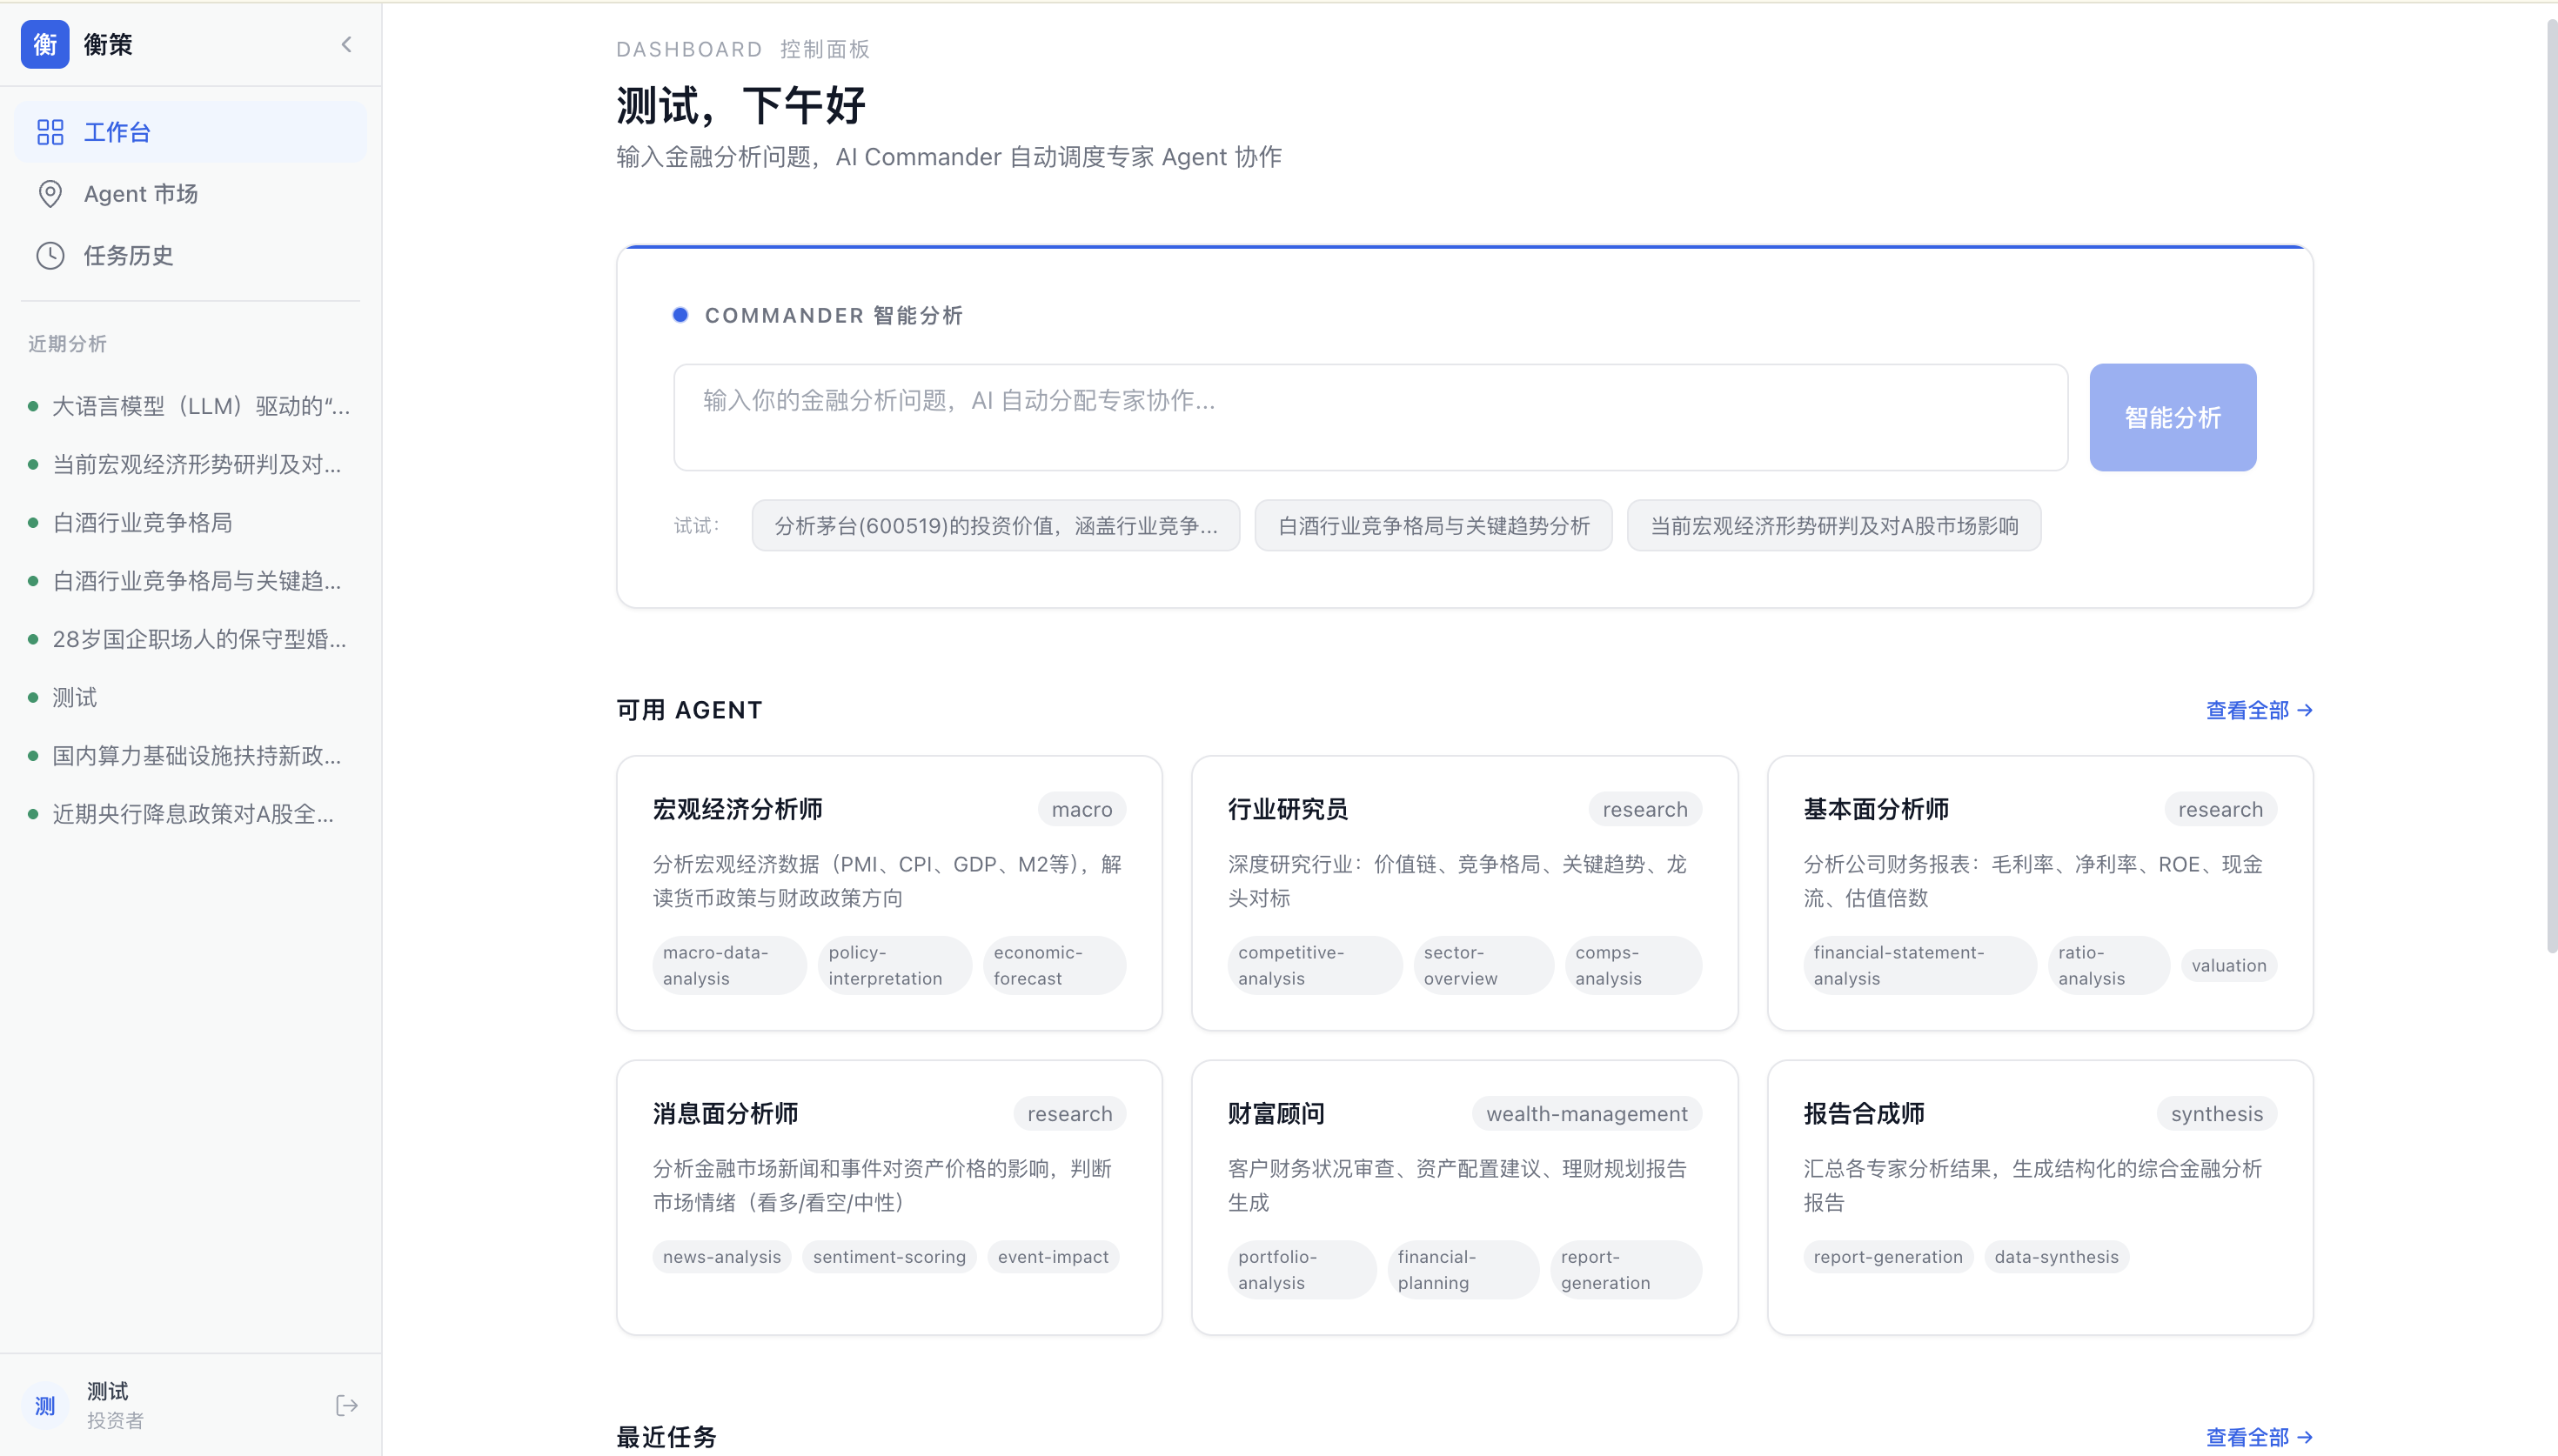
\includegraphics[keepaspectratio,alt={Dashboard首页 --- Commander输入与任务卡片}]{screenshots/demo1.png}}
\caption{Dashboard首页 --- Commander输入与任务卡片}
\end{figure}

\subsection{演示时刻 2：SSE
流式逐字推送（``我可以看着它思考''）}\label{ux6f14ux793aux65f6ux523b-2sse-ux6d41ux5f0fux9010ux5b57ux63a8ux9001ux6211ux53efux4ee5ux770bux7740ux5b83ux601dux8003}

每个 Agent 的分析结果是逐字出现在屏幕上的------不是等 2
分钟后一次性弹出，而是像打字机一样实时输出。4 个 Agent
的分析卡片同时更新，各卡片独立展示''正在分析中 /
已完成''状态，用户可以看到每一步推理过程。\textbf{这是技术含量的关键证据：SSE
协议的工程实现。}

\begin{figure}
\centering
\pandocbounded{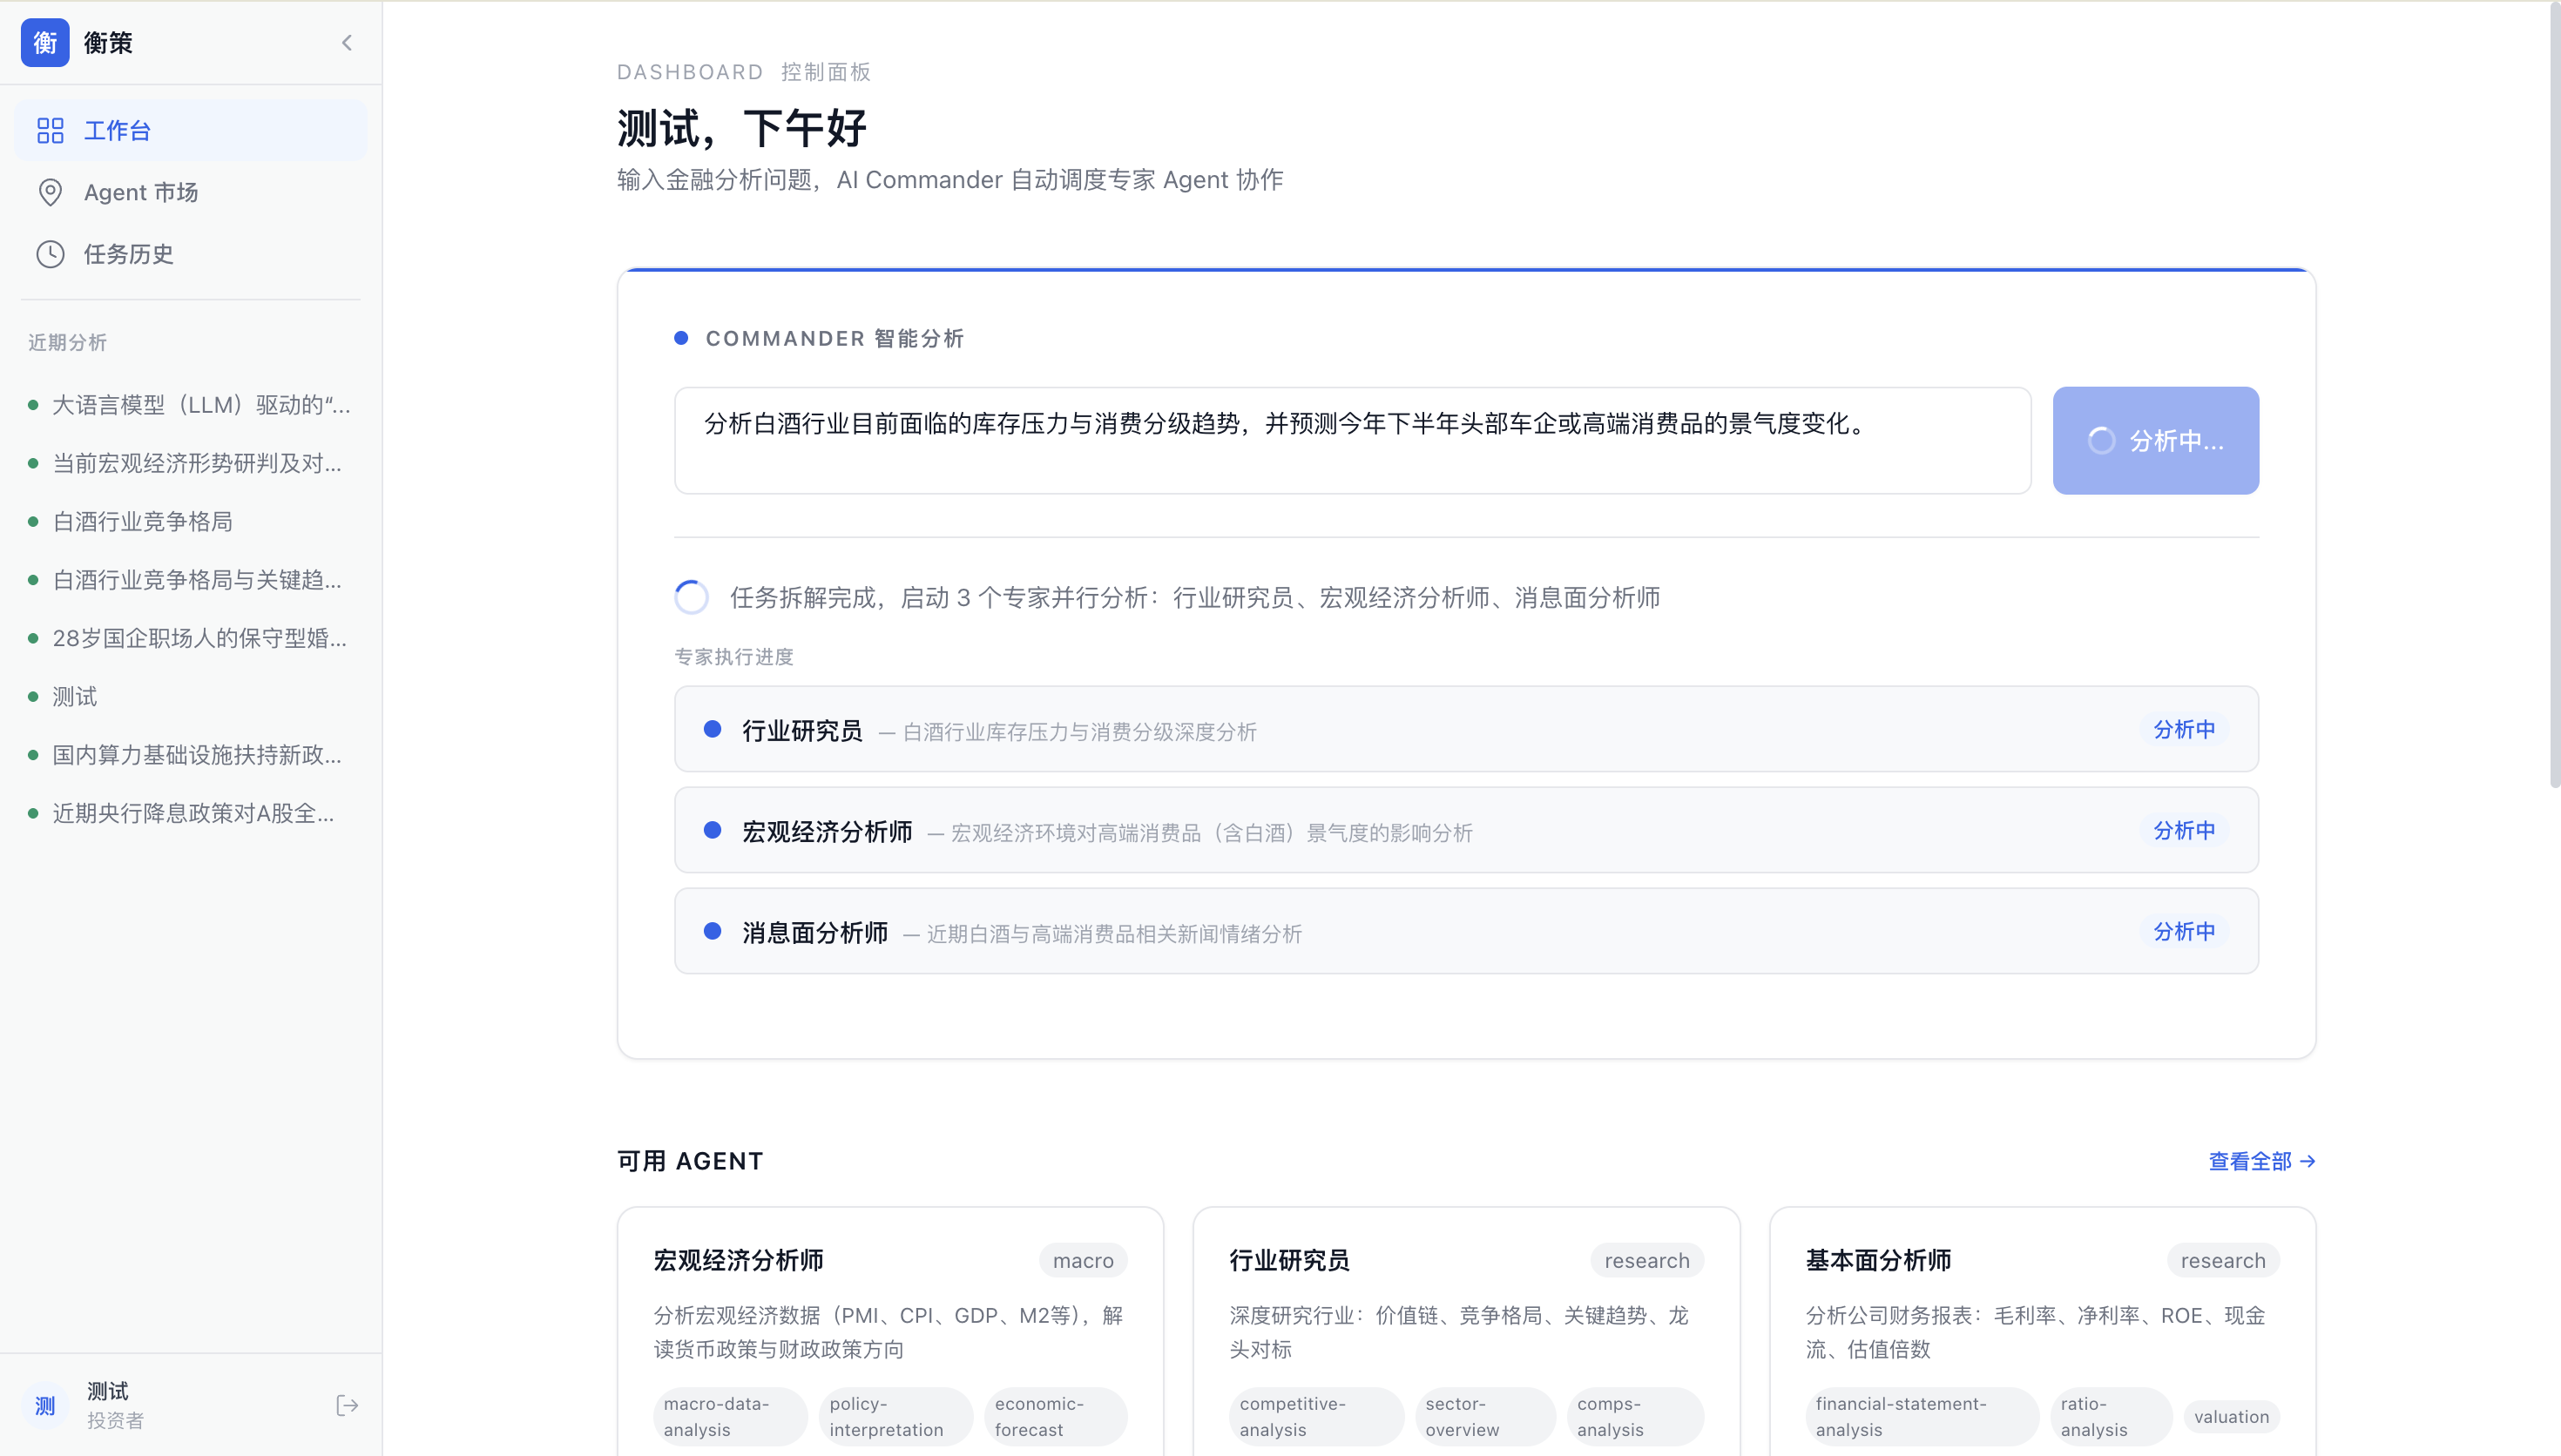
\includegraphics[keepaspectratio,alt={Commander编排中 --- 4个Agent并行分析，SSE实时推送}]{screenshots/demo2.png}}
\caption{Commander编排中 --- 4个Agent并行分析，SSE实时推送}
\end{figure}

\subsection{演示时刻
3：搜索引用蓝色链接（``结论不是它编的''）}\label{ux6f14ux793aux65f6ux523b-3ux641cux7d22ux5f15ux7528ux84ddux8272ux94feux63a5ux7ed3ux8bbaux4e0dux662fux5b83ux7f16ux7684}

综合报告页展示报告合成师整合的多维度分析结论。每条分析结论后面附有蓝色的搜索来源链接（如''来源：东方财富网''）。评委可以要求点击任一链接，跳转到原始网页进行验证。\textbf{这是回应''AI
可信度''质疑的最直接方式。}

\begin{figure}
\centering
\pandocbounded{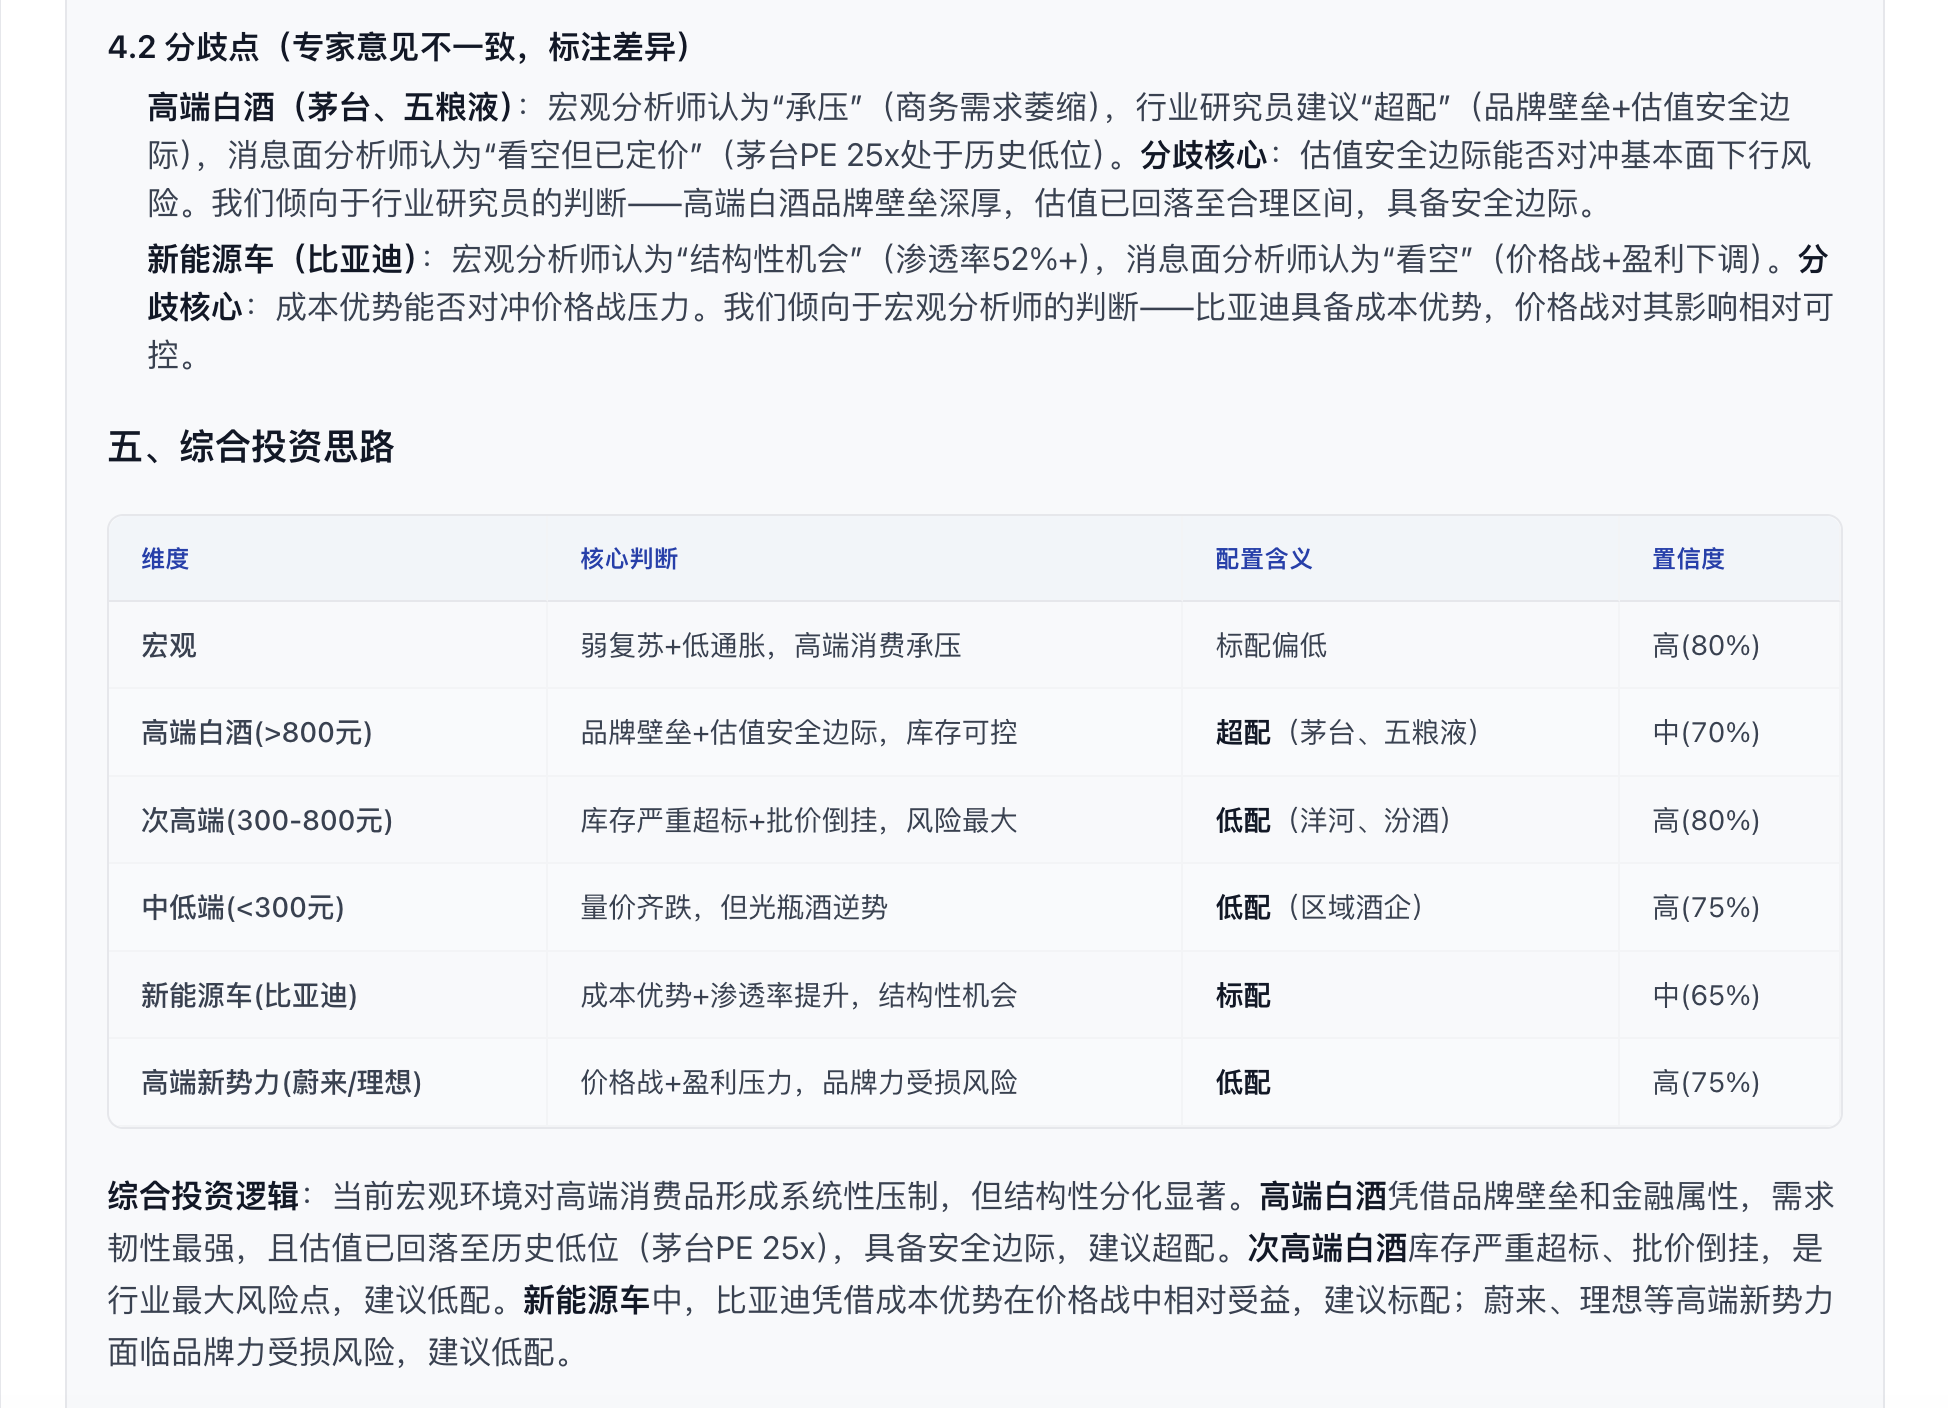
\includegraphics[keepaspectratio,alt={综合报告页（上）--- 多维度分析结论 + 搜索引用蓝色链接}]{screenshots/demo3.1.png}}
\caption{综合报告页（上）--- 多维度分析结论 + 搜索引用蓝色链接}
\end{figure}

\begin{figure}
\centering
\pandocbounded{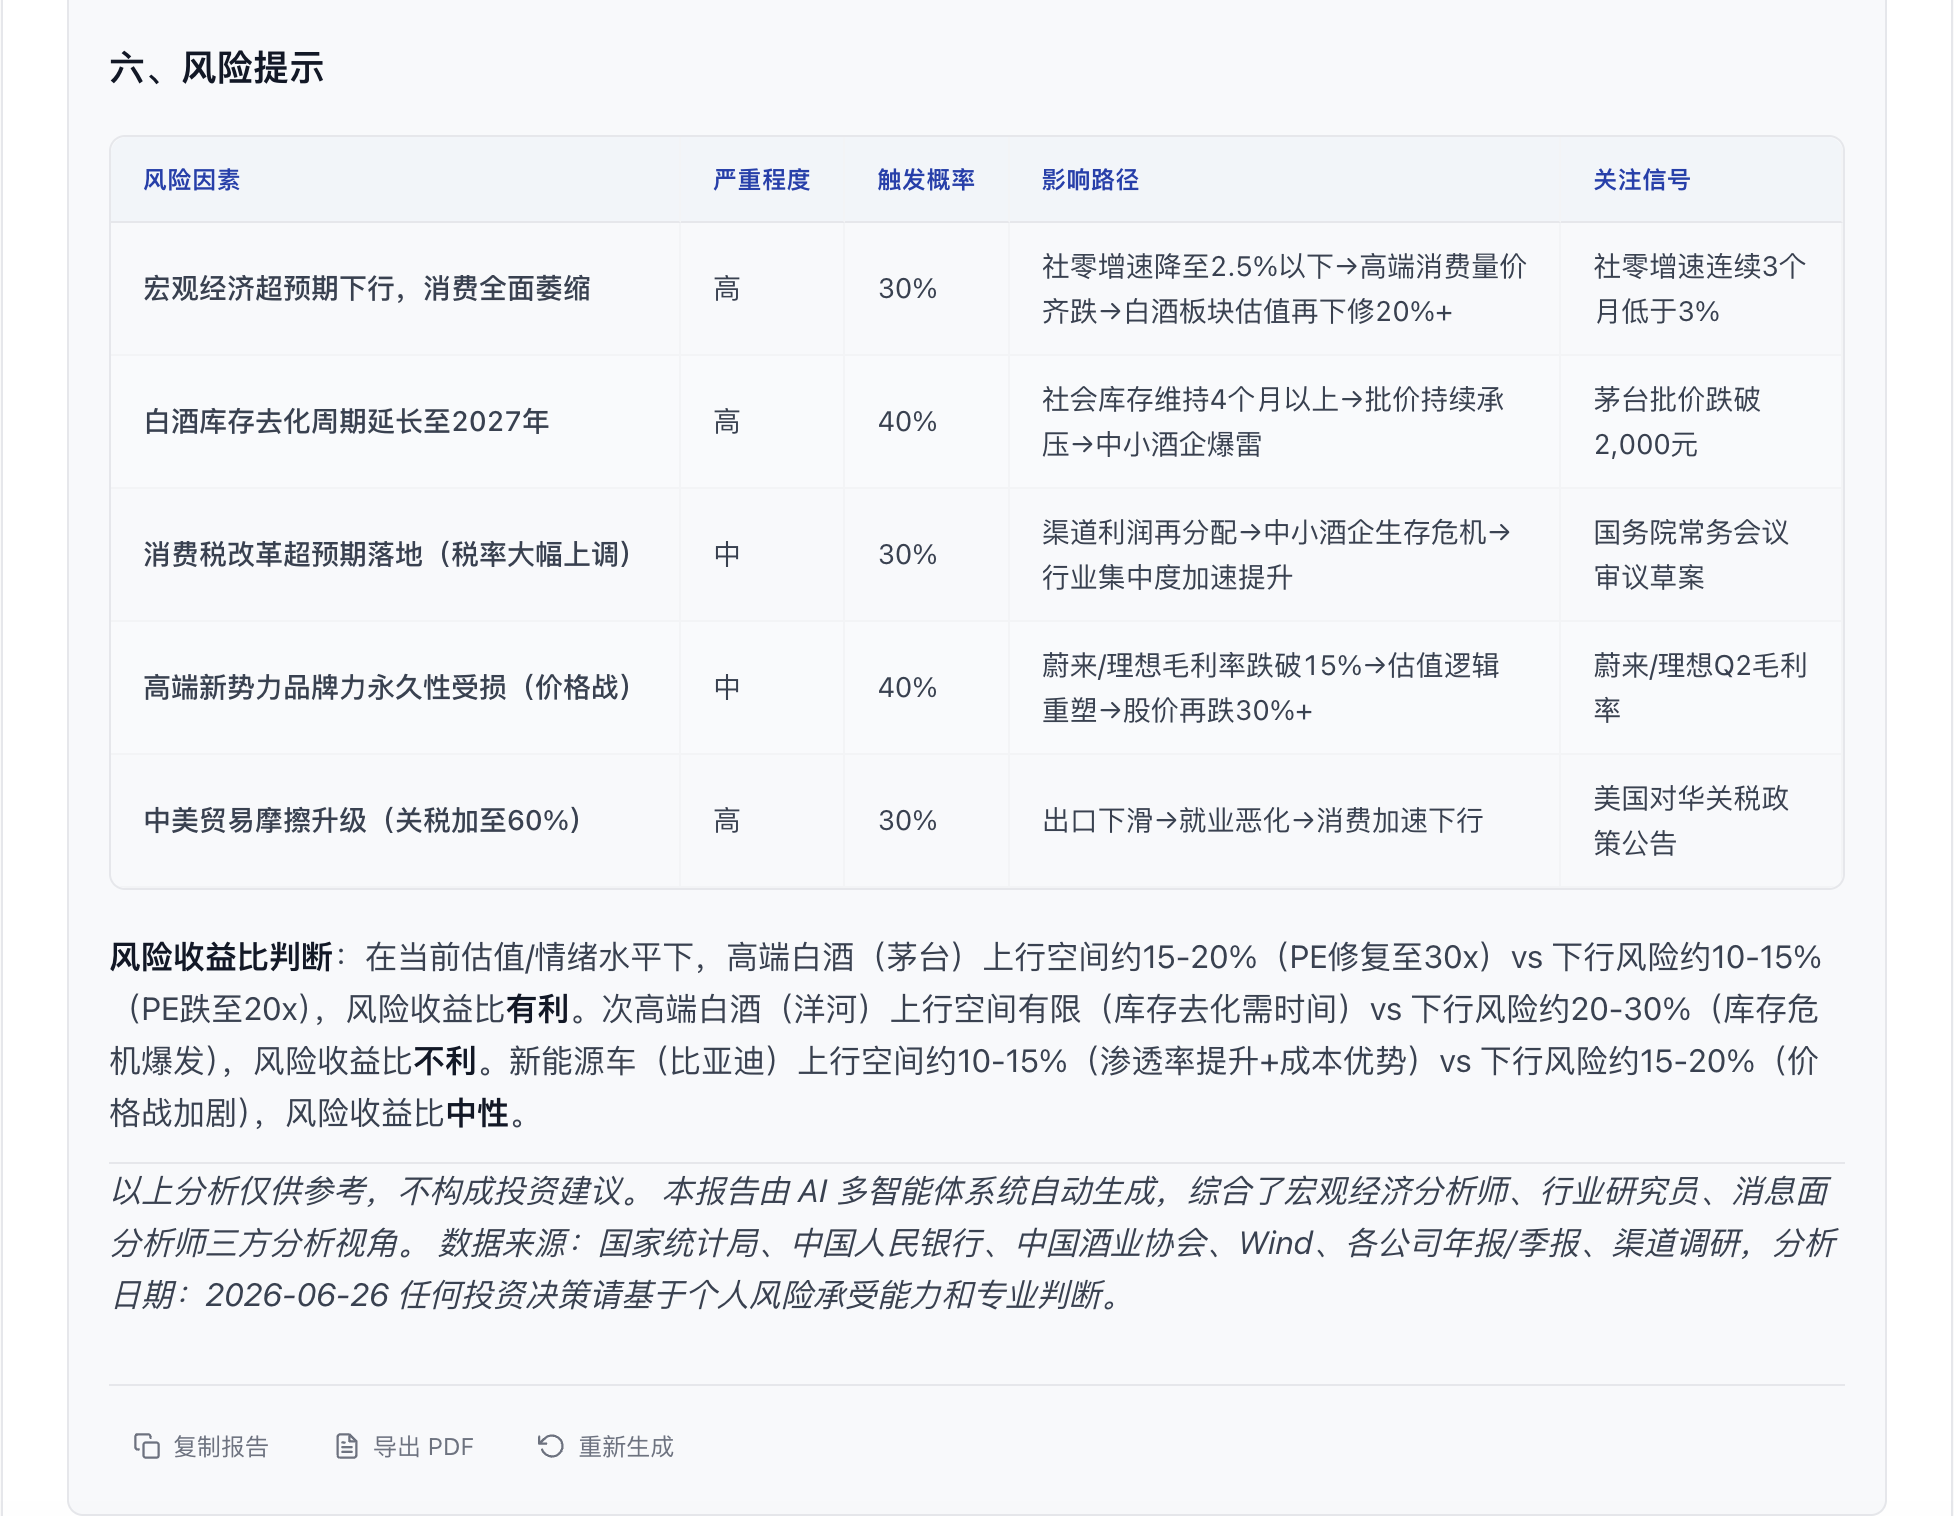
\includegraphics[keepaspectratio,alt={综合报告页（下）--- 报告尾部与操作按钮}]{screenshots/demo3.2.png}}
\caption{综合报告页（下）--- 报告尾部与操作按钮}
\end{figure}

\subsection{演示时刻 4：单 Agent
深度专项（``可以当专业工具用''）}\label{ux6f14ux793aux65f6ux523b-4ux5355-agent-ux6df1ux5ea6ux4e13ux9879ux53efux4ee5ux5f53ux4e13ux4e1aux5de5ux5177ux7528}

切换到单 Agent
模式，选择''宏观经济分析师''，输入''当前美联储降息周期对中国债市的影响''。展示
Agent
按照预设分析框架（GDP→CPI→M2→政策面→全球联动）逐项输出的结构化报告，包含宏观数据速览表、资产配置启示和风险矩阵。\textbf{展示
Agent 不只是''回答问题''，而是按专业方法论输出分析。}

\begin{figure}
\centering
\pandocbounded{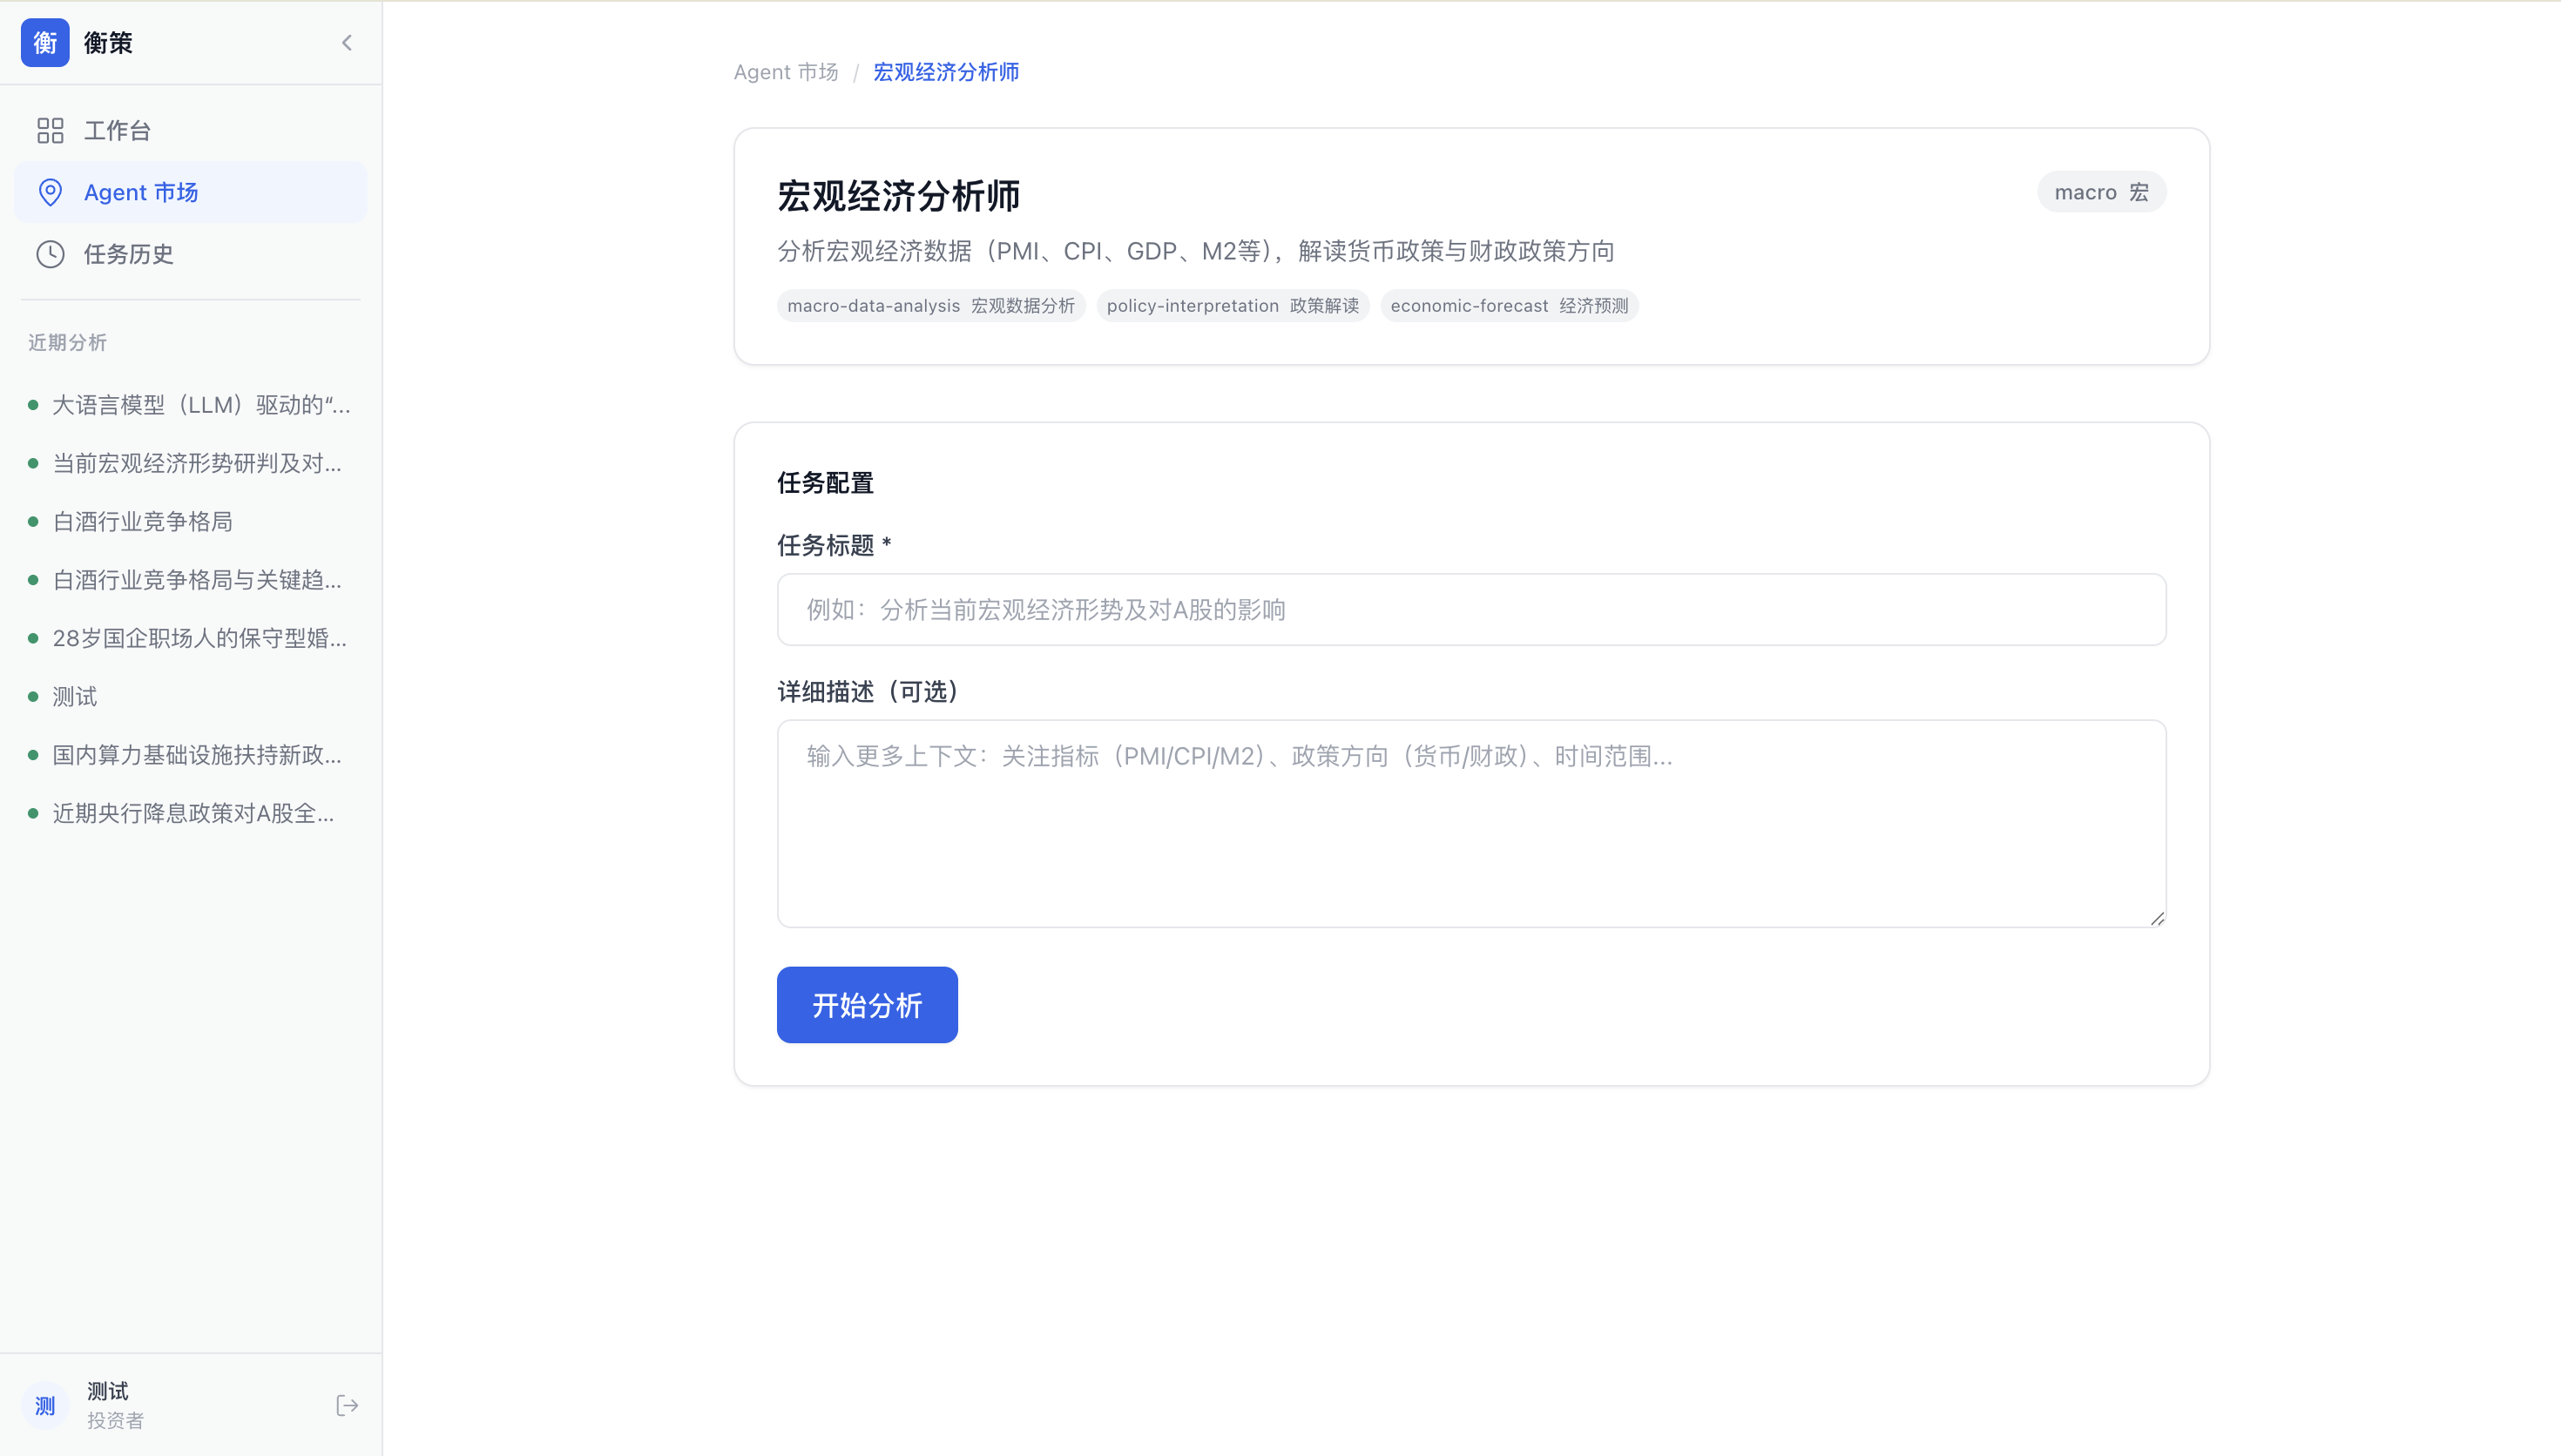
\includegraphics[keepaspectratio,alt={单Agent专项分析 --- 深度分析模式，流式逐字输出 + 搜索引用}]{screenshots/demo5.png}}
\caption{单Agent专项分析 --- 深度分析模式，流式逐字输出 + 搜索引用}
\end{figure}

\subsection{演示时刻 5：一键导出 PDF +
任务历史管理（``分析结果可以带走，可以回溯''）}\label{ux6f14ux793aux65f6ux523b-5ux4e00ux952eux5bfcux51fa-pdf-ux4efbux52a1ux5386ux53f2ux7ba1ux7406ux5206ux6790ux7ed3ux679cux53efux4ee5ux5e26ux8d70ux53efux4ee5ux56deux6eaf}

点击 PDF 导出按钮，综合报告在数秒内生成可打印的 PDF
文件。报告包含完整的表格、结论和来源链接。切换到任务历史页，展示所有存档的分析任务，支持查看历史报告、回溯中间结果和基于原参数重新运行。

\begin{figure}
\centering
\pandocbounded{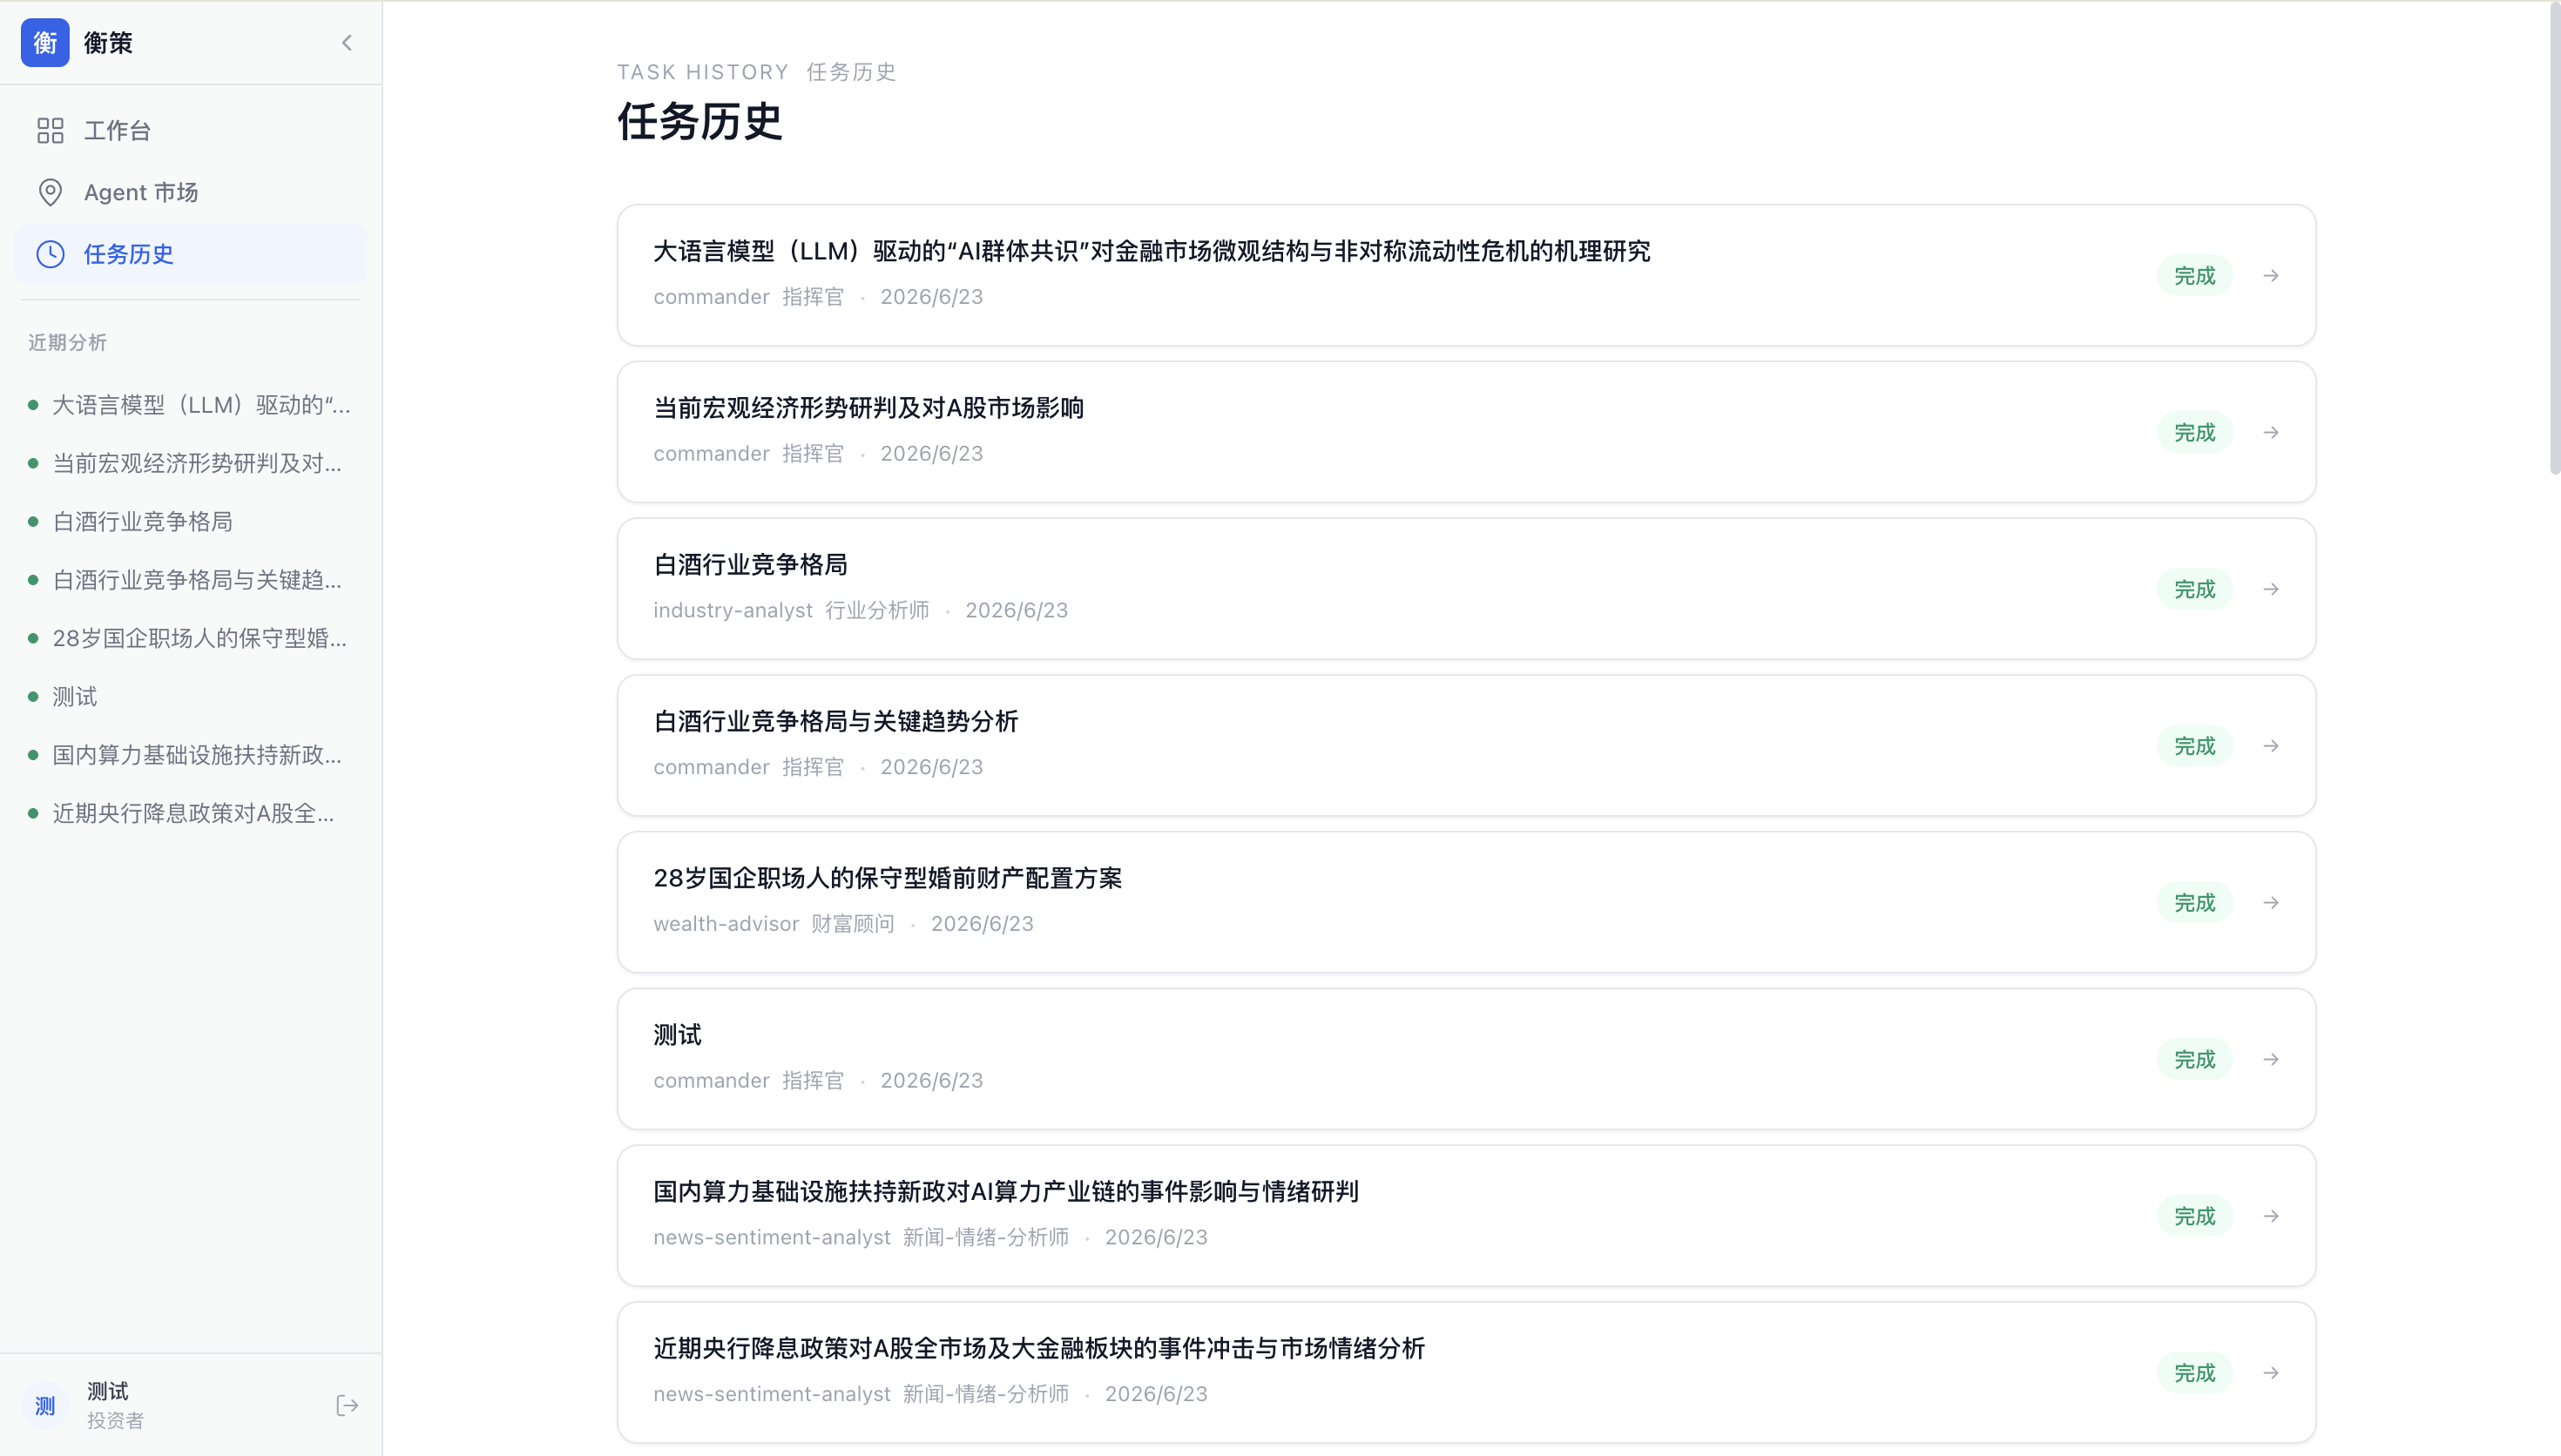
\includegraphics[keepaspectratio,alt={任务历史管理页 --- 分析任务存档列表}]{screenshots/demo6.png}}
\caption{任务历史管理页 --- 分析任务存档列表}
\end{figure}

\begin{figure}
\centering
\pandocbounded{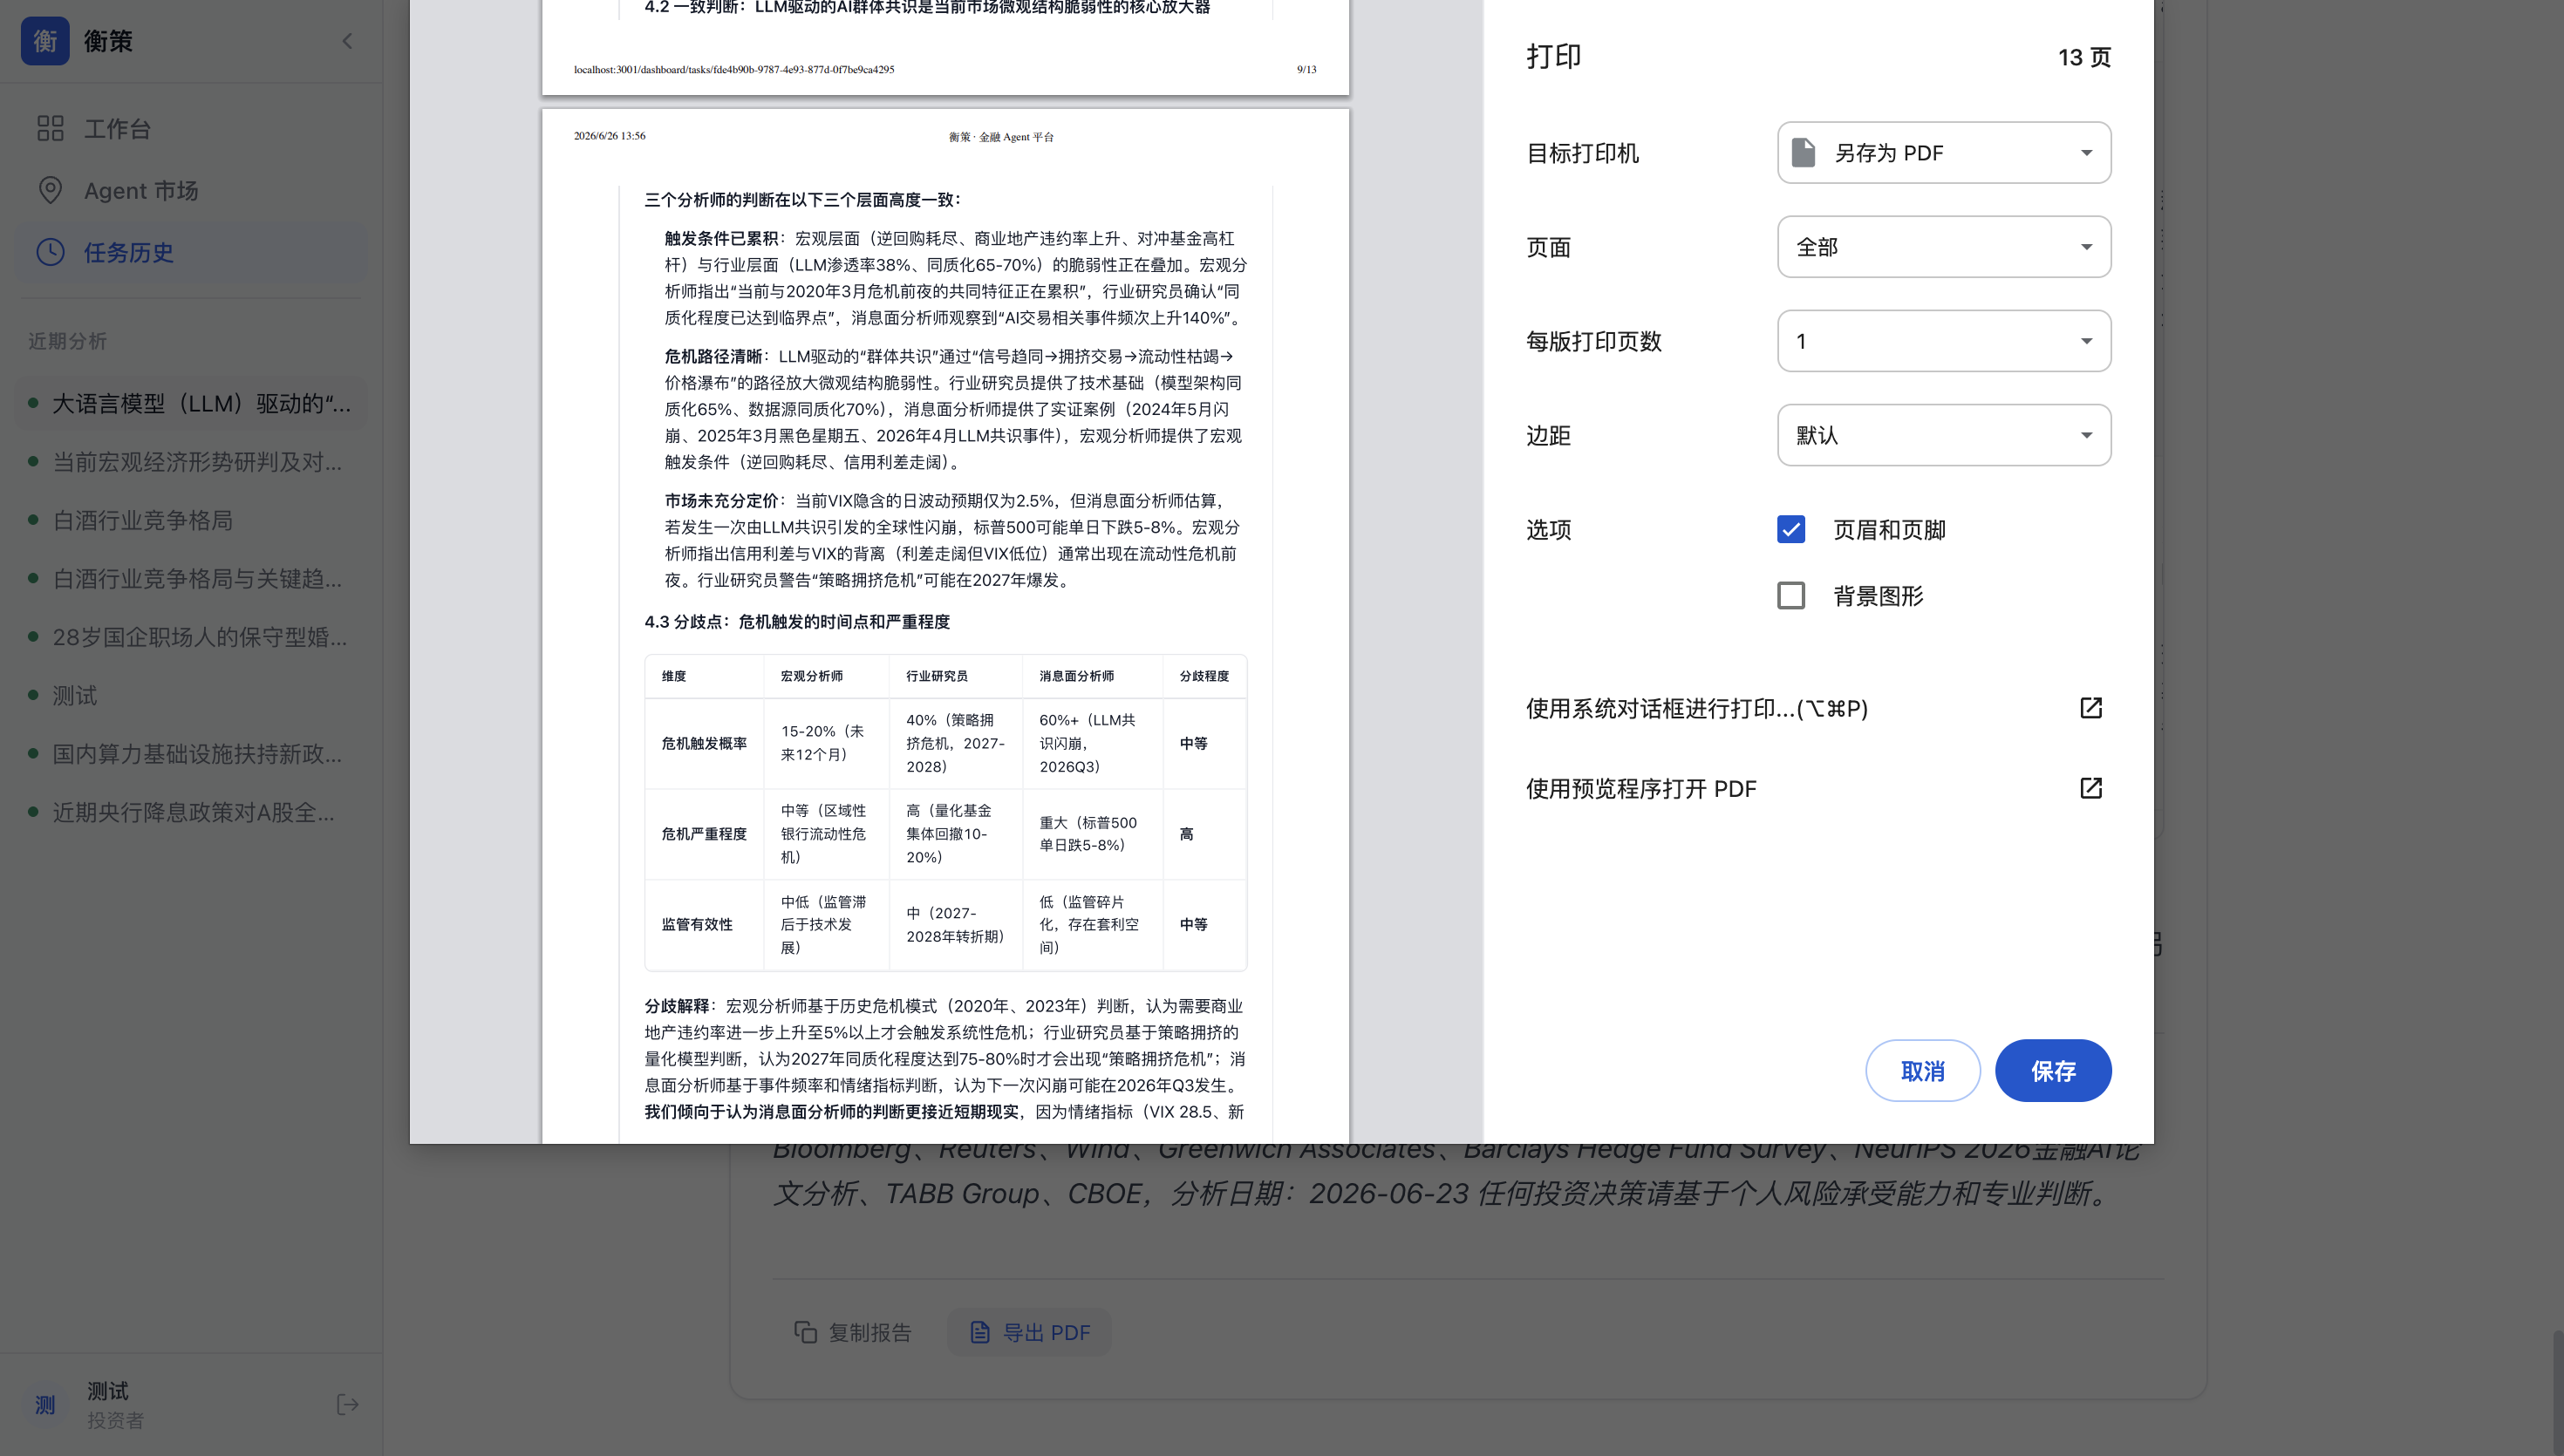
\includegraphics[keepaspectratio,alt={PDF导出 --- 报告一键导出，满足工作流闭环}]{screenshots/demo7.png}}
\caption{PDF导出 --- 报告一键导出，满足工作流闭环}
\end{figure}

\section{十一、实施路径与财务预算}\label{ux5341ux4e00ux5b9eux65bdux8defux5f84ux4e0eux8d22ux52a1ux9884ux7b97}

\subsection{（一）实施计划}\label{ux4e00ux5b9eux65bdux8ba1ux5212}

\begin{longtable}[]{@{}
  >{\raggedright\arraybackslash}p{(\linewidth - 6\tabcolsep) * \real{0.2143}}
  >{\raggedright\arraybackslash}p{(\linewidth - 6\tabcolsep) * \real{0.2143}}
  >{\raggedright\arraybackslash}p{(\linewidth - 6\tabcolsep) * \real{0.2857}}
  >{\raggedright\arraybackslash}p{(\linewidth - 6\tabcolsep) * \real{0.2857}}@{}}
\toprule\noalign{}
\begin{minipage}[b]{\linewidth}\raggedright
阶段
\end{minipage} & \begin{minipage}[b]{\linewidth}\raggedright
时间
\end{minipage} & \begin{minipage}[b]{\linewidth}\raggedright
里程碑
\end{minipage} & \begin{minipage}[b]{\linewidth}\raggedright
交付物
\end{minipage} \\
\midrule\noalign{}
\endhead
\bottomrule\noalign{}
\endlastfoot
\textbf{第一阶段：MVP 验证} & 已完成 & Commander + 6 Specialist
端到端跑通；SSE 实时流式；联网搜索引用；PDF 导出；SaaS 多用户；Docker
一键部署 & 可演示 MVP \\
\textbf{第二阶段：校赛打磨} & 当前 & 策划书撰写 + Demo 演示准备 +
功能稳定性优化 + 收集使用反馈 & 本策划书 + 6 张产品截图 \\
\textbf{第三阶段：数据层建设} & 校赛→省赛 & 接入 Tushare/东方财富 API
获取结构化金融数据；K 线/趋势图可视化；新增 4-6 个 Specialist；Agent
链式调用（依赖关系串行） & 数据增强版平台 \\
\textbf{第四阶段：智能层升级} & 省赛→全国赛 & RAG
知识库（研报/政策向量化检索）；WebSocket
实时双向推送；用户反馈收集机制；移动端适配 & 智能增强版平台 \\
\textbf{第五阶段：产品化} & 全国赛后 & 私有化部署方案完善；CI/CD +
自动化测试；API 限流 + 使用量统计；12+ Specialist Agent 矩阵 &
商业可部署版本 \\
\end{longtable}


\subsection{（二）技术路线图}\label{ux4e8cux6280ux672fux8defux7ebfux56fe}

\begin{verbatim}
当前（校赛 MVP）            →  省赛阶段                  →  全国赛/未来规划
─────────────────────────────────────────────────────────────────────────────
· Commander + 6 Specialist  · 接入真实金融数据源(Tushare)  · 12+ Specialist Agent 矩阵
· SSE 流式输出              · 新增 4-6 个 Specialist       · RAG 知识库（研报/政策向量化）
· 联网搜索引用              · Agent 链式调用(依赖关系)     · WebSocket 实时双向推送
· SaaS 多用户               · K 线/趋势图前端可视化        · 移动端适配
· PDF 一键导出              · 用户反馈收集机制             · K8s 生产部署 + CI/CD
· Docker 一键部署           · 数据脱敏 + 合规检查层        · 金融数据源多路接入
\end{verbatim}

\subsection{（三）财务预算}\label{ux4e09ux8d22ux52a1ux9884ux7b97}

\begin{longtable}[]{@{}
  >{\raggedright\arraybackslash}p{(\linewidth - 6\tabcolsep) * \real{0.2400}}
  >{\centering\arraybackslash}p{(\linewidth - 6\tabcolsep) * \real{0.2000}}
  >{\centering\arraybackslash}p{(\linewidth - 6\tabcolsep) * \real{0.2000}}
  >{\raggedright\arraybackslash}p{(\linewidth - 6\tabcolsep) * \real{0.3600}}@{}}
\toprule\noalign{}
\begin{minipage}[b]{\linewidth}\raggedright
项目
\end{minipage} & \begin{minipage}[b]{\linewidth}\centering
费用（校赛阶段）
\end{minipage} & \begin{minipage}[b]{\linewidth}\centering
费用（省赛阶段）
\end{minipage} & \begin{minipage}[b]{\linewidth}\raggedright
用途说明
\end{minipage} \\
\midrule\noalign{}
\endhead
\bottomrule\noalign{}
\endlastfoot
DeepSeek API 调用 & ¥200-500/月 & ¥500-2,000/月 &
模型推理费用（含联网搜索），按实际调用量计费 \\
云服务器 & ¥0（本地 Docker） & ¥100-300/月 & 生产环境部署 \\
金融数据源接入 & ¥0 & ¥0-500/月 & Tushare 社区版免费，增值版按需 \\
域名 + HTTPS & ¥0（本地） & ¥200-500/年 & 生产部署必备 \\
\textbf{合计} & \textbf{¥200-500/月} & \textbf{¥600-3,300/月} &
校赛阶段月成本 ¥300 以内，学生可承受 \\
\end{longtable}


\section{十二、附录}\label{ux5341ux4e8cux9644ux5f55}

\subsection{附录
A：技术栈详情}\label{ux9644ux5f55-aux6280ux672fux6808ux8be6ux60c5}

\begin{longtable}[]{@{}
  >{\raggedright\arraybackslash}p{(\linewidth - 4\tabcolsep) * \real{0.2857}}
  >{\raggedright\arraybackslash}p{(\linewidth - 4\tabcolsep) * \real{0.4286}}
  >{\raggedright\arraybackslash}p{(\linewidth - 4\tabcolsep) * \real{0.2857}}@{}}
\toprule\noalign{}
\begin{minipage}[b]{\linewidth}\raggedright
层次
\end{minipage} & \begin{minipage}[b]{\linewidth}\raggedright
技术选型
\end{minipage} & \begin{minipage}[b]{\linewidth}\raggedright
说明
\end{minipage} \\
\midrule\noalign{}
\endhead
\bottomrule\noalign{}
\endlastfoot
\textbf{前端} & Next.js 14 + TypeScript + Tailwind CSS & SSR
服务端渲染，Dashboard / Agent / 任务详情三主页面 \\
\textbf{后端} & Python 3.12 + FastAPI & RESTful API + SSE
流式端点，异步高性能 \\
\textbf{AI 引擎} & DeepSeek API（含原生联网搜索） &
模型自动判断是否搜索，返回引用来源 \\
\textbf{数据库} & PostgreSQL 16 + pgvector & 用户/任务/Agent 持久化 +
向量检索能力（预埋） \\
\textbf{缓存} & Redis 7 & Session 管理 + 热点数据 \\
\textbf{容器化} & Docker Compose & 一键启动全栈，开发/部署一致 \\
\textbf{数据协议} & MCP（Model Context Protocol） & Agent
间统一通信标准 \\
\textbf{Markdown 渲染} & ReactMarkdown + remark-gfm & 报告内容渲染 \\
\textbf{版本控制} & Git + GitHub & 源码管理 + 持续集成规划 \\
\end{longtable}


\subsection{附录
B：核心数据来源}\label{ux9644ux5f55-bux6838ux5fc3ux6570ux636eux6765ux6e90}

\begin{longtable}[]{@{}
  >{\raggedright\arraybackslash}p{(\linewidth - 2\tabcolsep) * \real{0.5000}}
  >{\raggedright\arraybackslash}p{(\linewidth - 2\tabcolsep) * \real{0.5000}}@{}}
\toprule\noalign{}
\begin{minipage}[b]{\linewidth}\raggedright
数据
\end{minipage} & \begin{minipage}[b]{\linewidth}\raggedright
来源
\end{minipage} \\
\midrule\noalign{}
\endhead
\bottomrule\noalign{}
\endlastfoot
金融大模型中标 587 项目 / 15.06 亿元 & 智能超参数 2025 年度报告 \\
2026 = ``金融智能体元年'' & 2026 年陆家嘴论坛（阿里云主题演讲） \\
工行 AI 员工年承担 5.5 万人年 / 科技投入 285.88 亿元 & 工商银行 2025
年度报告 \\
工行''数智工行（AI-ICBC）``战略 / 500+ 场景 & 工商银行 2026
年经营工作会议 \\
金融监管总局 AI 指导意见（2026.6） & 国家金融监督管理总局 \\
银行业 AI 中标占比 75.2\% & 智能超参数 2025 年度报告 \\
交易智能化比率 96\% & 工商银行 2025 年度报告 \\
平安集团部署智能体 5 万+ & 平安集团公开披露 \\
42 家 A 股上市银行九成已部署 AI & 各银行年报综合 \\
金融科技 AI 核心市场（2030E）6,200 亿元 & 艾瑞咨询 \\
\end{longtable}


\begin{quote}
\textbf{策划书撰写日期：2026 年 6 月 26 日}

\emph{弈金 --- 让 AI
从''一个聪明人''进化为''一支可以协作、可以审计、可以调度的数字分析团队''。}
\end{quote}

\end{document}
